\def\year{2022}\relax
%File: formatting-instructions-latex-2022.tex
%release 2022.1
\documentclass[letterpaper]{article} % DO NOT CHANGE THIS
\usepackage{aaai22}  % DO NOT CHANGE THIS
\usepackage{times}  % DO NOT CHANGE THIS
\usepackage{helvet}  % DO NOT CHANGE THIS
\usepackage{courier}  % DO NOT CHANGE THIS
\usepackage[hyphens]{url}  % DO NOT CHANGE THIS
\usepackage{graphicx} % DO NOT CHANGE THIS
\urlstyle{rm} % DO NOT CHANGE THIS
\def\UrlFont{\rm}  % DO NOT CHANGE THIS
\usepackage{natbib}  % DO NOT CHANGE THIS AND DO NOT ADD ANY OPTIONS TO IT
\usepackage{caption} % DO NOT CHANGE THIS AND DO NOT ADD ANY OPTIONS TO IT
\usepackage{color} % DO NOT CHANGE THIS AND DO NOT ADD ANY OPTIONS TO IT
\DeclareCaptionStyle{ruled}{labelfont=normalfont,labelsep=colon,strut=off} % DO NOT CHANGE THIS
\frenchspacing  % DO NOT CHANGE THIS
\setlength{\pdfpagewidth}{8.5in}  % DO NOT CHANGE THIS
\setlength{\pdfpageheight}{11in}  % DO NOT CHANGE THIS
%
% These are recommended to typeset algorithms but not required. See the subsubsection on algorithms. Remove them if you don't have algorithms in your paper.
\usepackage{algorithm}
\usepackage{algorithmic}

%
% These are are recommended to typeset listings but not required. See the subsubsection on listing. Remove this block if you don't have listings in your paper.
\usepackage{newfloat}
\usepackage{listings}
\lstset{%
	basicstyle={\footnotesize\ttfamily},% footnotesize acceptable for monospace
	numbers=left,numberstyle=\footnotesize,xleftmargin=2em,% show line numbers, remove this entire line if you don't want the numbers.
	aboveskip=0pt,belowskip=0pt,%
	showstringspaces=false,tabsize=2,breaklines=true}
\floatstyle{ruled}
\newfloat{listing}{tb}{lst}{}
\floatname{listing}{Listing}
\newcommand{\KZ}[1]{\textcolor{blue}{Kenny: #1}}
%
%\nocopyright
%
% PDF Info Is REQUIRED.
% For /Title, write your title in Mixed Case.
% Don't use accents or commands. Retain the parentheses.
% For /Author, add all authors within the parentheses,
% separated by commas. No accents, special characters
% or commands are allowed.
% Keep the /TemplateVersion tag as is
\pdfinfo{
/Title (AAAI Press Formatting Instructions for Authors Using LaTeX -- A Guide)
/Author (AAAI Press Staff, Pater Patel Schneider, Sunil Issar, J. Scott Penberthy, George Ferguson, Hans Guesgen, Francisco Cruz, Marc Pujol-Gonzalez)
/TemplateVersion (2022.1)
}

% added %%%%%%%%%%%%%%%%%%%%%%%%%%%%%%%%%%%%%%%%%%%%%%%% 
\usepackage{booktabs}
\usepackage{tikz}
\usetikzlibrary{arrows,shapes, decorations.pathmorphing,backgrounds,positioning}
\tikzset{every picture/.style={/utils/exec={\sffamily}}}
\usepackage{subcaption}
\usepackage{amsmath}
\usepackage{multirow}
% added %%%%%%%%%%%%%%%%%%%%%%%%%%%%%%%%%%%%%%%%%%%%%%%% 

% DISALLOWED PACKAGES
% \usepackage{authblk} -- This package is specifically forbidden
% \usepackage{balance} -- This package is specifically forbidden
% \usepackage{color (if used in text)
% \usepackage{CJK} -- This package is specifically forbidden
% \usepackage{float} -- This package is specifically forbidden
% \usepackage{flushend} -- This package is specifically forbidden
% \usepackage{fontenc} -- This package is specifically forbidden
% \usepackage{fullpage} -- This package is specifically forbidden
% \usepackage{geometry} -- This package is specifically forbidden
% \usepackage{grffile} -- This package is specifically forbidden
% \usepackage{hyperref} -- This package is specifically forbidden
% \usepackage{navigator} -- This package is specifically forbidden
% (or any other package that embeds links such as navigator or hyperref)
% \indentfirst} -- This package is specifically forbidden
% \layout} -- This package is specifically forbidden
% \multicol} -- This package is specifically forbidden
% \nameref} -- This package is specifically forbidden
% \usepackage{savetrees} -- This package is specifically forbidden
% \usepackage{setspace} -- This package is specifically forbidden
% \usepackage{stfloats} -- This package is specifically forbidden
% \usepackage{tabu} -- This package is specifically forbidden
% \usepackage{titlesec} -- This package is specifically forbidden
% \usepackage{tocbibind} -- This package is specifically forbidden
% \usepackage{ulem} -- This package is specifically forbidden
% \usepackage{wrapfig} -- This package is specifically forbidden
% DISALLOWED COMMANDS
% \nocopyright -- Your paper will not be published if you use this command
% \addtolength -- This command may not be used
% \balance -- This command may not be used
% \baselinestretch -- Your paper will not be published if you use this command
% \clearpage -- No page breaks of any kind may be used for the final version of your paper
% \columnsep -- This command may not be used
% \newpage -- No page breaks of any kind may be used for the final version of your paper
% \pagebreak -- No page breaks of any kind may be used for the final version of your paperr
% \pagestyle -- This command may not be used
% \tiny -- This is not an acceptable font size.
% \vspace{- -- No negative value may be used in proximity of a caption, figure, table, section, subsection, subsubsection, or reference
% \vskip{- -- No negative value may be used to alter spacing above or below a caption, figure, table, section, subsection, subsubsection, or reference

\setcounter{secnumdepth}{2} %May be changed to 1 or 2 if section numbers are desired.

% The file aaai22.sty is the style file for AAAI Press
% proceedings, working notes, and technical reports.
%

% Title

% Your title must be in mixed case, not sentence case.
% That means all verbs (including short verbs like be, is, using,and go),
% nouns, adverbs, adjectives should be capitalized, including both words in hyphenated terms, while
% articles, conjunctions, and prepositions are lower case unless they
% directly follow a colon or long dash
\iffalse
\title{AAAI Press Formatting Instructions \\for Authors Using \LaTeX{} --- A Guide}
\author{
    %Authors
    % All authors must be in the same font size and format.
    Written by AAAI Press Staff\textsuperscript{\rm 1}\thanks{With help from the AAAI Publications Committee.}\\
    AAAI Style Contributions by Pater Patel Schneider,
    Sunil Issar,\\
    J. Scott Penberthy,
    George Ferguson,
    Hans Guesgen,
    Francisco Cruz\equalcontrib,
    Marc Pujol-Gonzalez\equalcontrib
}
\affiliations{
    %Afiliations
    \textsuperscript{\rm 1}Association for the Advancement of Artificial Intelligence\\
    % If you have multiple authors and multiple affiliations
    % use superscripts in text and roman font to identify them.
    % For example,

    % Sunil Issar, \textsuperscript{\rm 2}
    % J. Scott Penberthy, \textsuperscript{\rm 3}
    % George Ferguson,\textsuperscript{\rm 4}
    % Hans Guesgen, \textsuperscript{\rm 5}.
    % Note that the comma should be placed BEFORE the superscript for optimum readability

    2275 East Bayshore Road, Suite 160\\
    Palo Alto, California 94303\\
    % email address must be in roman text type, not monospace or sans serif
    publications22@aaai.org
%
% See more examples next
}
\fi

%Example, Multiple Authors, ->> remove \iffalse,\fi and place them surrounding AAAI title to use it
\title{Modeling Multi-level Context for Informational Bias Detection by 
Contrastive Learning and Sentential Graph Network}
% \author {
%     % Authors
%     Shijia Guo,\textsuperscript{\rm 1}
%     Kenny Q. Zhu, \textsuperscript{\rm 1}
% }
% \affiliations {
%     % Affiliations
%     \textsuperscript{\rm 1} Shanghai Jiao Tong University\\
%     % \textsuperscript{\rm 2} Affiliation 2\\
%     seveny1997@sjtu.edu.cn, kzhu@cs.sjtu.edu.cn
% }

%Example, Single Author, ->> remove \iffalse,\fi and place them surrounding AAAI title to use it
\iffalse
\title{My Publication Title --- Single Author}
\author {
    Author Name
}
\affiliations{
    Affiliation\\
    Affiliation Line 2\\
    name@example.com
}
\fi


\begin{document}

\maketitle

\begin{abstract}
Informational bias is widely present in news articles. 
It refers to providing one-sided, selective or suggestive information of specific aspects of certain entity to guide a specific interpretation, thereby biasing the reader's opinion. Sentence-level informational bias detection is a very challenging task in a way that such bias can only be revealed together with the context, examples include collecting information from various sources or analyzing the entire article in combination with the background. In this paper, we integrate three levels of context to detect the sentence-level informational bias in English news articles: adjacent sentences, whole article, and articles from other news outlets describing the same event. Our model, MultiCTX (Multi-level ConTeXt), uses contrastive learning and sentence graphs together with Graph Attention Network (GAT) to encode these three degrees of context at different stages by tactically composing contrastive triplets and constructing sentence graphs within events. Our experiments proved that contrastive learning together with sentence graphs effectively incorporates context in varying degrees and significantly outperforms the current SOTA model sentence-wise in informational bias detection.

\end{abstract}





\section{Introduction}


\KZ{You need to emphasize that the event-level context is critical for this
particular application: news bias detection.}
Informational bias broadly exists in news articles. As a sort of framing bias, it always frames a certain entity by specific aspects using narrow, speculative or indicative information  to guide a particular interpretation, thus swaying readers' opinion. 

For most of us, news articles are the main source of information. Therefore, news articles play a central role in shaping individual and public opinions. However, news reports often show internal bias. The current research is often limited to the lexical bias. This form of bias rarely depends on the context of the sentence. It can be eliminated by deleting or replacing a small number of biased words. Contrarily, researchers \citet{fan-etal-2019-plain} found that the informational bias is more common and more difficult to detect.
% among which informational bias is found to be one of the most common and difficult to detect.

Different from other types of bias, the detection of informational bias depends on a large extent of the context. This fact makes the sentence-level informational bias detection a very challenging task. A sentence alone can be expressed in a neutral manner, but it might be revealed as biased in consideration of the context. Take the second row in Table \ref{tab:basil} as example: the sentence \textit{``Mr. Mattis, a retired four-star Marine general, was rebuffed.''} \label{sent:mattis} seems to be a simple declarative sentence stating a fact. However, if we read the previous sentence (the first row in Table \ref{tab:basil}) , we will know that \textit{`a retired four-star Marine general'} indicates a negative, even ironic tone towards Mr. Mattis and his last attempt. Therefore, sentence-level informational bias can only be revealed by collecting information from various sources and analyzing the entire article together with its background. Such subtleties of informational bias are more likely to affect unsuspecting readers, which indicates the necessity of research into new detection methods. 

In this paper, we propose MultiCTX (Multi-level ConTeXt), a model composed of contrastive learning and sentence graph attention networks to encode three different levels of context:  \textbf{1) Neighborhood-context}: adjacent sentences, i.e. sentences in the same article around the target sentence; \textbf{2) Article-context}: the whole article containing the target sentence; \textbf{3) Event-context}: articles from various news media reporting the same event. These three levels encompass the contextual information from the most local to the most global.

In order to make use of the context rather than be overwhelmed by the noise introduced, MultiCTX prioritizes contrastive learning which learns sentence embedings via discriminating among $(target, positive$ $sample, negative$ $sample)$ triplets to distill the essence of the target sentence. The quality of the learned CSE (Contrastive Sentence Embedding) relies on that of triplets. Other than the traditional brute-force way to select triplets only based on their labels, MultiCTX further considers article-level information which creates higher-quality triplets. Such triplet formulation guarantees that our CSEs infuse the context and reflect sentences' inherent semantics instead of the shallow lexical features. 

% Work by \citet{baly-etal-2020-detect} used triplet loss instead of contrastive learning,
% directly within batch 
% Given a dataset of 0/1-labeled sentences, MultiCTX first construct tactically triplets from them. 

MultiCTX then builds a relational sentence graph using CSEs. Edges are connected between two sentences if they are logically related in the same \textit{neighborhood} or if they are continuous in entities or semantically similar within the same \textit{event}. Finally we apply a Self-supervised Graph Attention Network (SSGAT) on our sentence graph to make the final informational bias prediction. The SSGAT structure encodes neighborhood-level and event-level context via edges, making it possible for textually distant but contextually close sentences to connect directly. The flexible graph structure extends beyond the sequential arrangement of traditional LSTMs, which also consider the surrounding context. 

Although document graphs are not rare in NLP tasks, they are often short and built by token-wise dependency parsing. It may suffer from high complexity and considerable noise when applied on long texts which is our case with news articles. Our relational sentence graph uses sentence nodes and focuses on inter-sentence relationships. It recquires only minimal syntax parsing, takes on less noise and has better interpretability.


Few research studies sentence-level informational bias detection by infusing context. \citet{fan-etal-2019-plain} first published a human-annotated dataset on this task, taking the context into account during annotation. However, sentences are still treated sentences individually in their model. \citet{van-den-berg-markert-2020-context} did a primary research on incorporating different levels of context in the informational bias detection. However, they consider only one kind of context in each model. To our best knowledge, our model is the first to incorporate multi-level contextual information in sentence-level classification task.
%  and their results are still not very satisfactory even compared to our ablation models using only one level of context as well

In summary, we present the following contributions:

\begin{itemize}
  \item We are the first to incorporate three different levels of context together in the sentence-level bias detection task. 
  \item We propose a novel triplet formation for contrastive learning in bias detection. The methodology can be generalized for other tasks.
  \item We are the first to use a sentence graph to encode the textual context information in the bias detection task.
  \item Our model MultiCTX significantly outperforms the current state-of-the-art model by 2 percentage points F1 score. It indicates that contextual information effectively helps sentence-level informational bias detection and our model successfully infuses multi-level context.
\end{itemize}

% The rest of our paper is organized as follows:



% - 我做的分别的也比别人做的好



% These three levels cover, from the closest to the furthest, from the most local to the most global, and from the most specific to most general.

% Intuitively, informational bias in a sentence can only be revealed by collecting information from various sources or analyzing the entire article in combination with the background. 


%  Our experiments proved that contrastive learning together with sentence graph effectively incorporates context in varying degrees and significantly outperforms the current SOTA model in informational bias detection.









% - use forward reference
% - yiyi




\section{Data and event-based Splitting}
\KZ{I still think that this section should go into experiments and 
be called ``Data set and implementation details''. If you want to give intuition
of why you split by the events, u can say so in that section. Don't give ppl
the impression that you are designing your approach based on this dataset.
In fact how you split the data is not that important. I actually think that to
make a stronger case, you need to experiment on at least another data set.
If you can't find any, can you label some more using some other newspapers?}
 We use BASIL (Bias Annotation Spans on the
 Informational Level) dataset proposed by \citet{fan-etal-2019-plain}. BASIL dataset provides sentence-by-sentence span-level annotation of informational bias for 300 English news articles grouped in 100 triplets, each discussing on the same event from three news outlets. The articles are selected in order to make a fair coverage in terms of time and ideology: 1) From 2010 to 2019, 10 events are included each year in the dataset; 2) Fox News (FOX), New York Times (NYT) and Huffington Post (HPO), representative of conservative, neutral and liberal respectively in the US journalism, are chosen as three news sources.
% \begin{itemize}
%     \item From 2010 to 2019, 10 events are included each year in the dataset
%     \item Fox News (FOX), New York Times (NYT) and Huffington Post (HPO), representative of conservative, neutral and liberal respectively in the US journalism, are chosen as three news sources.
% \end{itemize}
% Follow \citet{fan-etal-2019-plain} and \citet{van-den-berg-markert-2020-context},

As for the sentence-level informational bias detection task, we use the same data formulation in \citet{van-den-berg-markert-2020-context}. In this sentence-wise binary classification task, a sentence is labeled as biased if at least one informational bias span occurs, and seven empty sentences are removed, resulting in a total of 7977 sentences with 1221 annotated bias.

Furthermore, different from the commonly-used data splitting which randomly distributes sentences to one of the three subsets (train/val/test), we use event-wise data splitting mentioned in \citet{van-den-berg-markert-2020-context}, \citet{chen-etal-2020-detecting}. We treat each triplet reporting the same event as a unit and keeping sentences from the same event in the same subset. 

This cross-event splitting is intuitively in line with the nature of news reports and the way people learn about the world in real life: news articles emerge almost simultaneously in large numbers along with a particular event, over which people reason based on their experience. Moreover, people usually read an article as a whole instead of randomly picking up several sentences. They tend to collect information from more than one article to get a bigger picture of the new event. Therefore, splitting by events is more reasonable and more demanding, in terms of model generalizability for identifying informational bias from unseen events. (See Table \ref{tab:basil}.)
% Experiments in \citet{van-den-berg-markert-2020-context} and \citet{chen-etal-2020-detecting} also show that common models including BERT-based models all experienced a considerable performance drop when switching from random splitting to event-based splitting. 

% Examples are shown in Table \ref{tab:basil}.

\begin{table*}[th]
    \centering
	\scriptsize
    \begin{tabular}{cccp{12cm}c}
        \toprule[2pt]
        \textbf{Event} & \textbf{Source} & \textbf{Index} & \textbf{Sentence} & \textbf{Label} \\
        \midrule[1pt]
        86 & nyt & 3 &  Officials said Mr. Mattis went to the White House with his resignation letter already written, but nonetheless made a last attempt at persuading the president to reverse his decision about Syria, which Mr. Trump announced on Wednesday over the objections of his senior advisers. & 0\\
        \hline
        86 & nyt & 4 &  Mr. Mattis, a retired four-star Marine general, was rebuffed. & 1\\
        \hline
        86 & nyt & 5 &  Returning to the Pentagon, he asked aides to print out 50 copies of his resignation letter and distribute them around the building. & 0 \\
        \midrule
        11 & fox & 20 & However, Democrats rejected the plan even before Trump announced it, and a Senate version of the plan failed to get the 60 votes needed on Thursday.  & 1\\
\hline
        11 & fox & 21 & A second bill, already passed by the Democrat-controlled House to re-open the government, also fell short. & 0\\
        \midrule
        2 & hpo & 10 & There were roughly 520,000 arrests for unauthorized border crossings last year, which is about one-third of the 1.6 million arrests that happened in 2000. & 0\\
        \hline
        2 & hpo & 11 &Since 2014, a high proportion of those crossing have been Central American children and families seeking to make humanitarian claims such as asylum. & 1\\
        \bottomrule[2pt]
    \end{tabular}
    \caption{BASIL dataset}
    \label{tab:basil}
\end{table*}
        % 92 & hpo & 1 & WASHINGTON -- Massachusetts Gov. Deval Patrick (D) on Wednesday appointed William Mo Cowan to the Senate seat vacated by newly confirmed Secretary of State John Kerry. & 0\\
        % \hline
        % 92 & hpo & 2 & Cowan will hold the seat in an interim capacity until an election in June. & 0\\
        % \hline
        % 92 & hpo & 3 & Patrick, Cowan and Lt. Governor Tim Murray were all smiles as they walked into a news conference to announce the appointment. & 1\\
        % \hline
        % 51 & fox & 0 & Kathy Griffin admitted Tuesday she "went too far" on her latest photo shoot with controversial photographer Tyler Shields in which she is holding a bloodied mask of President Trump. & 0\\
        % \hline
        % 51 & fox & 1 & The gory photo first published in TMZ from Griffin's photo session with the famed Shields, known for his shocking pictures.& 1\\
        % \hline
        % 51 & fox & 2 & In a Twitter post late Tuesday, Griffin said the image "is too disturbing," and that "it wasn't funny." & 0\\
        % \hline

% People always face a new event around which a cluster of / plenty of reports emerge altogether/in batches.

% the emergence of cluster of news reports is event-driven / reports occur in event wise,, as well as people's perception of the world.

% develop views
% get a bigger picture of a new event.

% 模拟人学习新事件
% 人们学新的事物的时候是不会有可能的标签的

% 人们看文章的时候一篇看完且要多看几篇

% 人们对新事件的认知来自于这些related的新闻
% 时间上来说(news nature) 新的news一般会有很多文章一起出来因此unlabeled
% 人类学习来说 每次去认识一个新事件

% Keeping sentences from same event 
% sentence-wise event-wise

% assign distribute divide partition
% subsets division partitions parts

% splitting event-wise rather than sentence-wise
% 之前关于 BASIL 语料库的工作采用随机划分句子形成训练(training)、验证(validation)和测试集(test)(Fan 等,2019)。 这种类型的划会分将目标句子与同一文章中的其他句子以及涵盖同一事件的其他文章分别划分到不同集合。 以这种方式跨集合划分句子不符合实际生活中人们获取新闻报道的方式:同一事件的新闻报道总是几乎在同一时间出现,而人们也通常会整体地阅读一篇文章而非从中随机抽取几个句子浏览;况且,将同一文章中的句子分布在训练和测试数据中可以被视为一种泄漏,因为知道文章中的某些句子有偏见可能有助于识别同一文章或同一主题的另一篇文章中的相似句子 . 因此,我们采用按照事件进行划分,即同一事件下地三篇文章总是同时出现在同一集合中,这不仅更符合现实,更对模型的泛化能力提出更高要求,即要求能识别从未出现过的新的事件中的信息偏差。


% 人类获取信息的习惯
% 信息泄露
% 更好的泛化能力

% When we 

% Since context information is intuitively essential, and ideal model should be able to generalize to any kind of 



% generalization, leakage,xxxx
% Table 1 describes the BASIL dataset. 

\section{Methodology}
% \KZ{Here you can give a task description, which generalizes the BASIL dataset.
% You can say what is the input and output, that it being a binary classification
% problem etc. You can give one or two examples from Table 1 and leave the rest to
% experiment sec.}
Figure \ref{fig:model} illustrates our model MultiCTX (Multi-level ConTeXt). First, we carefully construct triplets from the original dataset and then apply supervised contrastive learning on them to obtain sentence embeddings. Second, we build relational sentence graphs by joining sentence nodes according to their discourse relationships and semantic similarity. Finally, we apply a Self-supervised Graph Attention Network \citep{kim2021how} to perform the bias detection as a node classification task. In essence, MultiCTX has two modules, Contrastive Learning Embedding (CSE) and Self-supervised Sentence Graph Attention Network (SSGAT).

\subsection{Sentence Embedding using Contrastive Learning}

The idea of contrastive learning is that humans discriminate objects by ``comparison'', thus similar objects should be close to each other in the representation space, and different objects should be as far apart as possible. However, news sentences inherently have small differences in terms of pure text. Two sentences with opposite stances might be different in a few words, while two sentences expressing the
same idea are likely to be formulated completely differently. To address the problem, we apply supervised contrastive learning with hard negatives described in \citet{gao2021simcse}. The idea is to develop, from the original dataset, the triplets $(x_i,x^+_i,x^-_i)$  each denotes target sentence, positive sample and negative sample respectively. Using the $\mathbf{h}_{i},\mathbf{h}_{i^+},\mathbf{h}_{i}^-$ representations of $x_i,x^+_i,x^-_i$, 
the objective function to minimize is InfoNCE Loss. 

% \begin{align}
% l_i = -\log \frac{e^{\operatorname{sim}\left(\mathbf{h}_{i}, \mathbf{h}_{i}^{+}\right) / \tau}}{\sum\limits_{j=1}^{\text{batch size}}\left(e^{\operatorname{sim}\left(\mathbf{h}_{i}, \mathbf{h}_{j}^{+}\right) / \tau}+e^{\operatorname{sim}\left(\mathbf{h}_{i}, \mathbf{h}_{j}^{-}\right) / \tau}\right)}
% \end{align}

The difficulty is to mine the positive and negative samples for each target sentence from the original dataset. A good positive sample is supposed to capture the most essential features of the sentence, rather than being influenced by other factors, such as the writing styles of different news media. Therefore, the best positive sample is expected to be significantly different from the target sample in terms of sentence formation, while the best negative sample should be similar to the target sentence in terms of syntactic structure. In short, samples with different labels from the target sentence but with initial embedding in its vicinity are likely to be the most useful, providing significant gradient information during the training process.

Inspired by \citet{baly-etal-2020-detect} which applies a triplet loss in training using news media in triplet selection, our final triplet follows article-based criteria and is composed of: $x_i$: target sentence; $x_i^+$: same label and event with $x_i$, but from a different article; $x_i^-$: from the same article with $x_i$ but with a different label. 

Thereby we essentially augment the original 7977-sentence BASIL corpus to a much larger dataset of around 300k triplets where sentences are no longer isolated but linked to two others. More importantly, triplets with the same target sentence provide altogether a 'context' to help its representational learning. This context integrates two advantages: 1) it provides article-level contextual information from the same article by the negative sample, and also event-level context from other articles of the same event; 2) it discourages the model to learn from superficial writing styles of the article or the news publisher. Our experiments also confirmed that this article-based triplet construction is better than either the news outlet-based triplet or the event-based one.

%  which achieves data enhancement in a certain sense. Moreover, since the ternary set is constructed using news articles under the same event (negative samples from the same article, and positive samples from different news sources but the same event), the model can not only exclude the influence of different news media writing styles in the process of comparative learning, and learn more essential content beyond rhetorical sentence construction, but also learn the contextual knowledge of the event described by the target text. This process simulates the process of receiving news and making judgments in the real world.




% 说一下按比例分布?有多少数据点?
% 画个图(降维之后)?
% In addition, in order to make the training samples cover the whole training set, this study constructs a sampling distribution that proportionalizes the sampling frequency to the number of available positive and negative samples to ensure that the final triad distribution is similar to the distribution of the original dataset.

% \begin{figure}[!htbp]\centering
%     \begin{tikzpicture}
%       [scale=.5, transform shape, 
%       event/.style = {rectangle,rounded corners, minimum width=230pt, minimum height = 140pt, draw = black, fill = white, thick},
%       vertex/.style = {rounded rectangle, minimum width=60pt, minimum height = 17pt, draw=red!50, fill = red!10, thick},
%       article/.style = {rectangle,rounded corners,minimum width=60pt, minimum height = 80pt, draw = orange!50, fill = orange!10, thick}, 
%       neg/.style = {rounded rectangle, minimum width=60pt, minimum height = 10pt, draw=blue!50, fill = blue!10, thick},
%       textbox/.style = {rectangle, minimum width=60pt, minimum height = 20pt},
%       edge_style/.style={draw=black, ultra thick}]
%       \node[event][fill=white] (n0) at (3,4)  {};
%       \node[textbox] at (2.6,2) {\large triplet $(x_i,x^+_i,x^-_i)$};
      
%       \node[article] (n1) at (1,4)  {};
%       \node[textbox] at (1,5) {article 1};
      
%       \node[article] (n2) at (4.5,4.5)  {};
%       \node[textbox] at (4.5,5.5) {article 3};

%       \node[article] (n3) at (5,3.5)  {};
%       \node[textbox] at (5,4.5) {article 2};
%       \node[vertex] (n4) at (1,4.5)  { $x_i^{ }$ };
%       \node[neg] (n5) at (1,3.2)  { $x_i^-$ };
%       \node[vertex] (n6) at (5,3.5)  { $x_i^+$ };
%       \node[textbox] at (-0.3,6) {event A};
%       \foreach \from \to /\weight in {n4/n5/,n4/n6/}
%         \draw[edge_style] (\from) -- node {\weight}(\to);
   
%     \end{tikzpicture}
%   \caption{Triplet construction. Positive sample $x_i^+$ has same label (red) and event with target sentence $x_i$; negative sample $x_i^-$ has different label (blue) but from the same article with $x_i$; note that three sentences must from same event.}
%   \label{fig:triplet}
% \end{figure}

% The difficulty of triplet loss is to mine the hard sampling. Take character recognition as an example: the same person, with different posture, or dress change, this is the hard positive sample. Two different people, wearing the same clothes and shooting from the same angle, is a hard negative sample.

% The purpose is to reduce the distance between similar things and increase the distance between different classes, so as to obtain a better representation vector for the text.

% by minimizing $\max (D(h,h^+)-D(h,h^-)+\alpha,0)$
% The performance of the sentence embedding obtained through contrastive learning is better already than that of BERT and LSTM by directly bifurcating it with the most basic logistic regression.

\subsection{Relational Sentence Graph}

Sentences are naturally suitable as nodes when encoding long documents, so we borrowed the idea from extractive text summarization from \citet{christensen-etal-2013-towards} and \citet{summpip} to construct graphs. The graphs are formed by connecting the sentences in four different ways:

\begin{enumerate} \label{para:edge}
    \item Deverbal noun reference: when an action in verb form occurs in the current sentence, it is likely to be mentioned in the noun form in the following sentences. So we attach the current sentence with its downstream sentence when at least one semantically similar deverbal noun is found in the latter.
    
    \item Discourse marker: If the immediately subsequent sentence begins with a discourse marker (e.g., however, meanwhile, furthermore), the two sentences are linked.
    
    \item Entity continuation: we connect two sentences in the same event if they contain the same entity.
    
    \item Sentence similarity: sentence pairs in the same event with high cosine similarity are joined.
    
\end{enumerate}

% 画个图,从真实数据里找句子, 找个event画一下 yes
% edge typeeeeeeeeeeeeeeeeeeeeeeee

\begin{figure}[!htbp]\centering
%   \begin{subfigure}[t]{0.7\linewidth}
%     \resizebox{\linewidth}{!}{
%     \begin{tikzpicture}
%       [scale=.6, transform shape,
%       vertex/.style = {rounded rectangle, minimum width=60pt, minimum height = 17pt, draw = black!30, thick},
%       textbox/.style = {rectangle, minimum width=60pt, minimum height = 20pt},
%       edge_style/.style={draw=black, ultra thick}]
%         \node[vertex] (n2) at (2,6)  {\textcolor{blue!60}{The inauguration will be held very soon.} };
%     \node[vertex] (n3) at (3,2)  { .... \textbf{Trump} has also...};
%       \node[vertex][draw=blue!60, fill = blue!40] (n4) at (1,3.5)  { \textcolor{white}{\textbf{Donald Trump} is \underline{elected} president }};
%       \node[vertex] (n5) at (-2,1.7)  { \textit{However}, there's... };
%       \node[vertex] (n6) at (6,5)  {...won the \underline{election}... };
%     %   \node[textbox] at (4.5,1.3) {event A};
%       \foreach \from \to /\weight in {n4/n5/}
%         \draw[draw=black] (\from) -- node {\weight}(\to);
%     \foreach \from \to /\weight in {n4/n6/}
%         \draw[draw=black, double distance=.03cm] (\from) -- node {\weight}(\to);
%   \foreach \from \to /\weight in {n4/n2/}
%         \draw[draw=blue!60] (\from) -- node {\weight}(\to);
%   \foreach \from \to /\weight in {n4/n3/}
%         \draw[edge_style] (\from) -- node {\weight}(\to);
%     \end{tikzpicture}}
%   \caption{\scriptsize Four types of edges in relational sentence graph. \underline{Underline}: deverbal noun reference; \textit{italic}: discourse maker; \textbf{bold}: entity continuation; \textcolor{blue!60}{colored}: sentence similarity}
%   \end{subfigure}
  \begin{subfigure}[t]{.35\linewidth}
    \resizebox{\linewidth}{!}{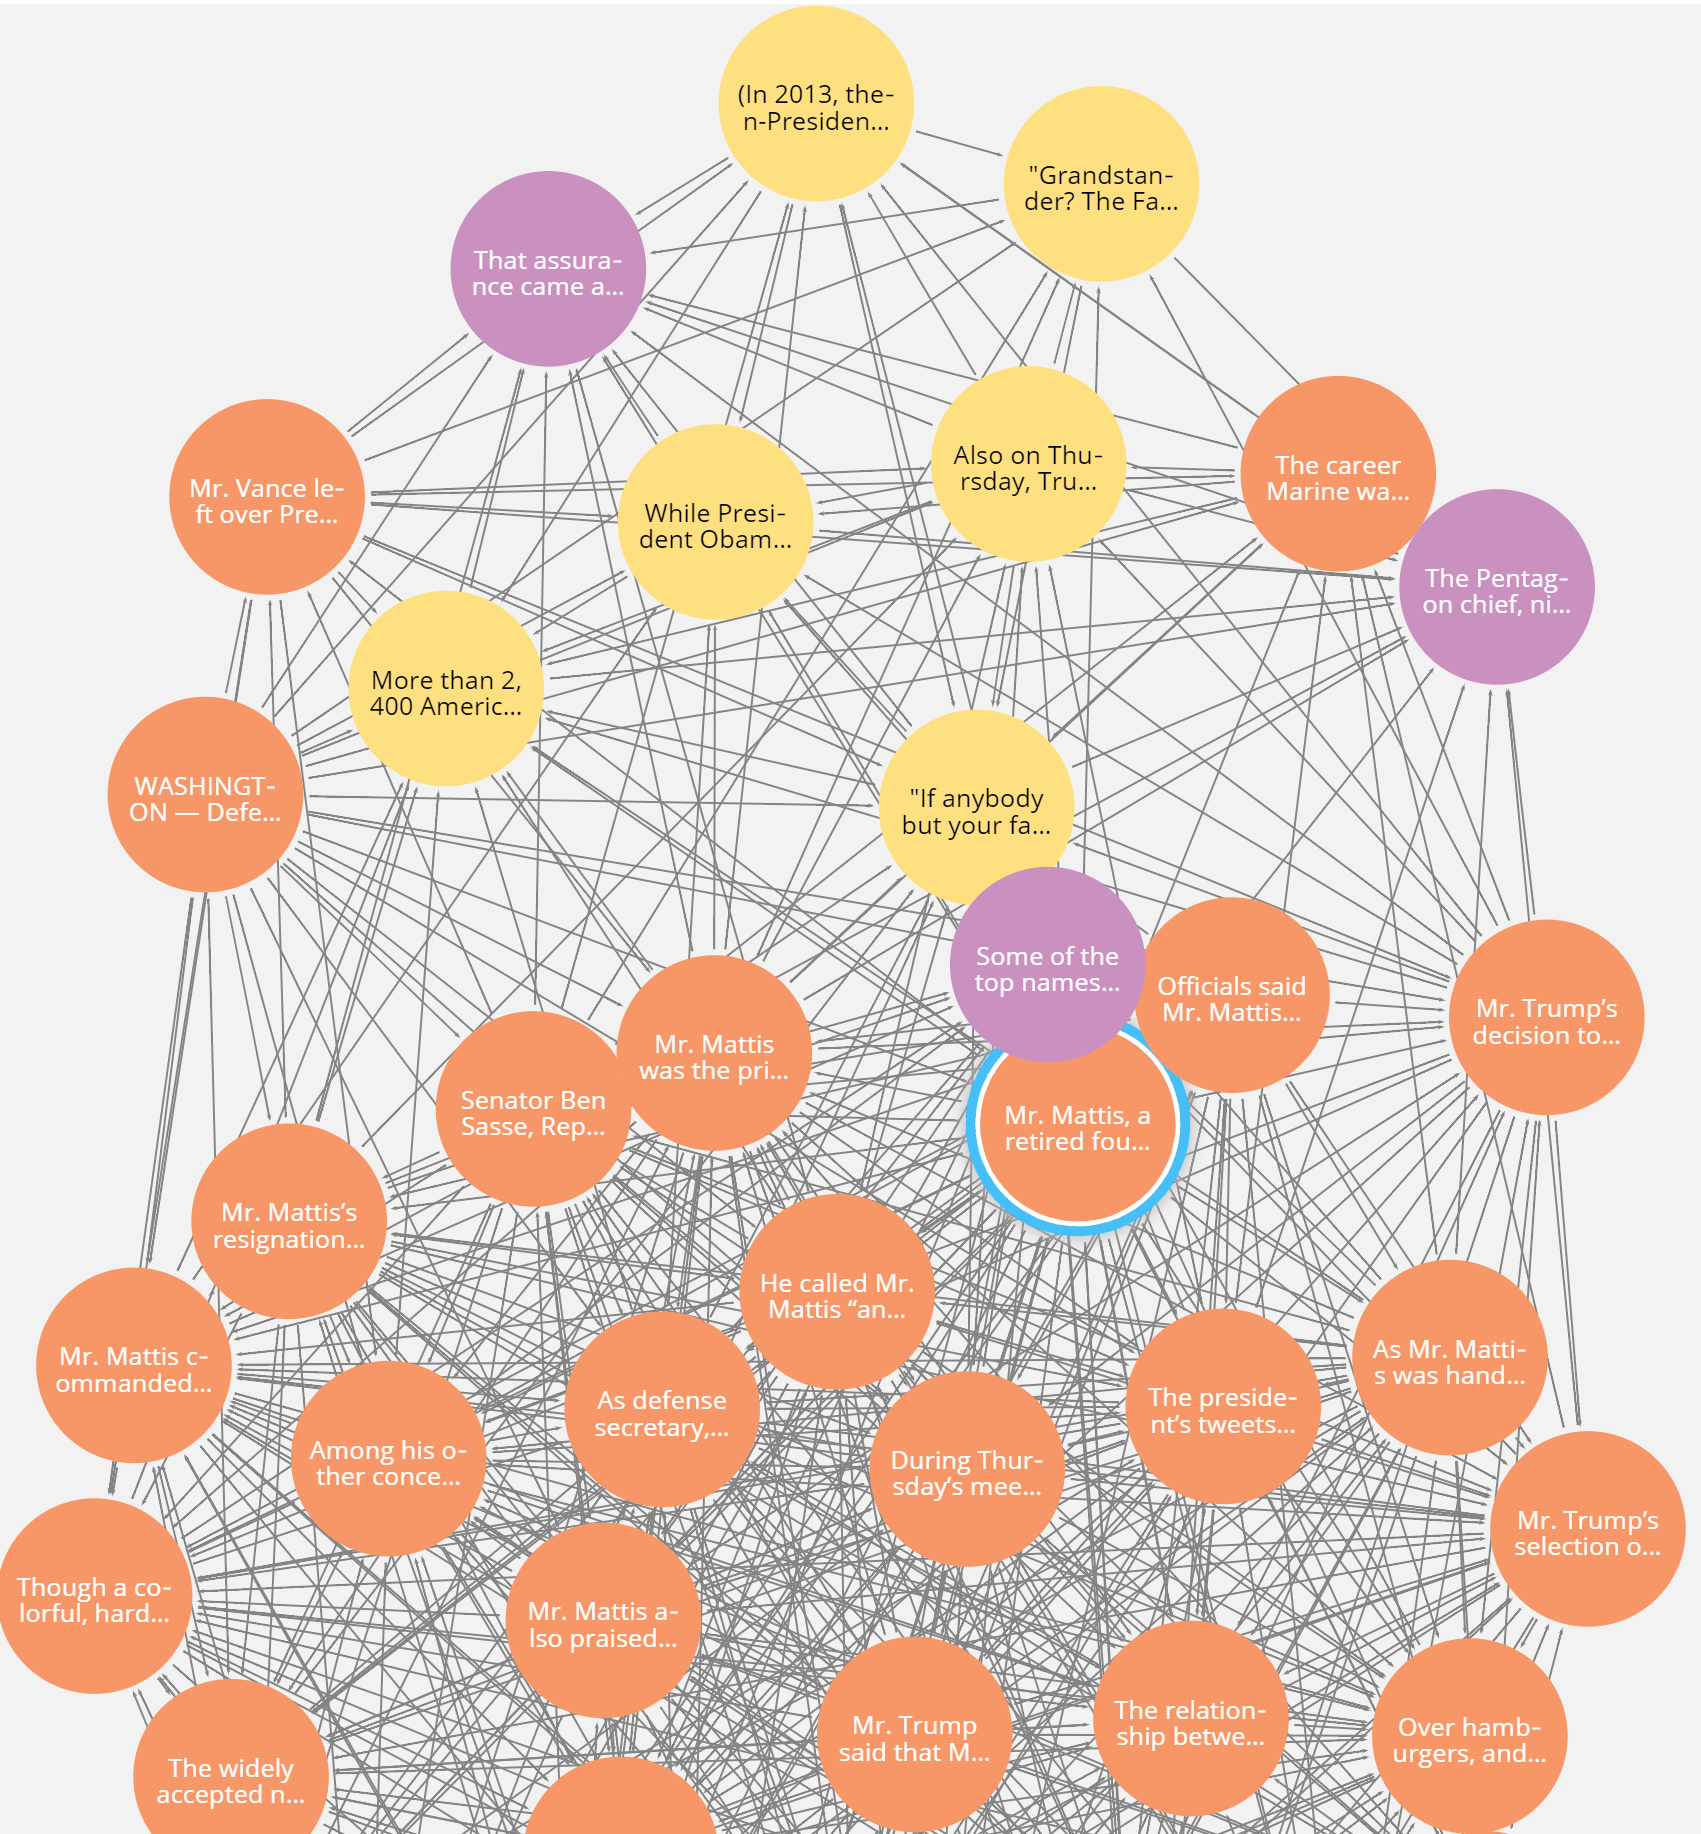
\includegraphics[]{img/mattis0_src.png}}
    \caption{\scriptsize nodes are colored by news source.}
    \label{subfig:mattissrc}
  \end{subfigure}
  \begin{subfigure}[t]{.35\linewidth}
    \resizebox{\linewidth}{!}{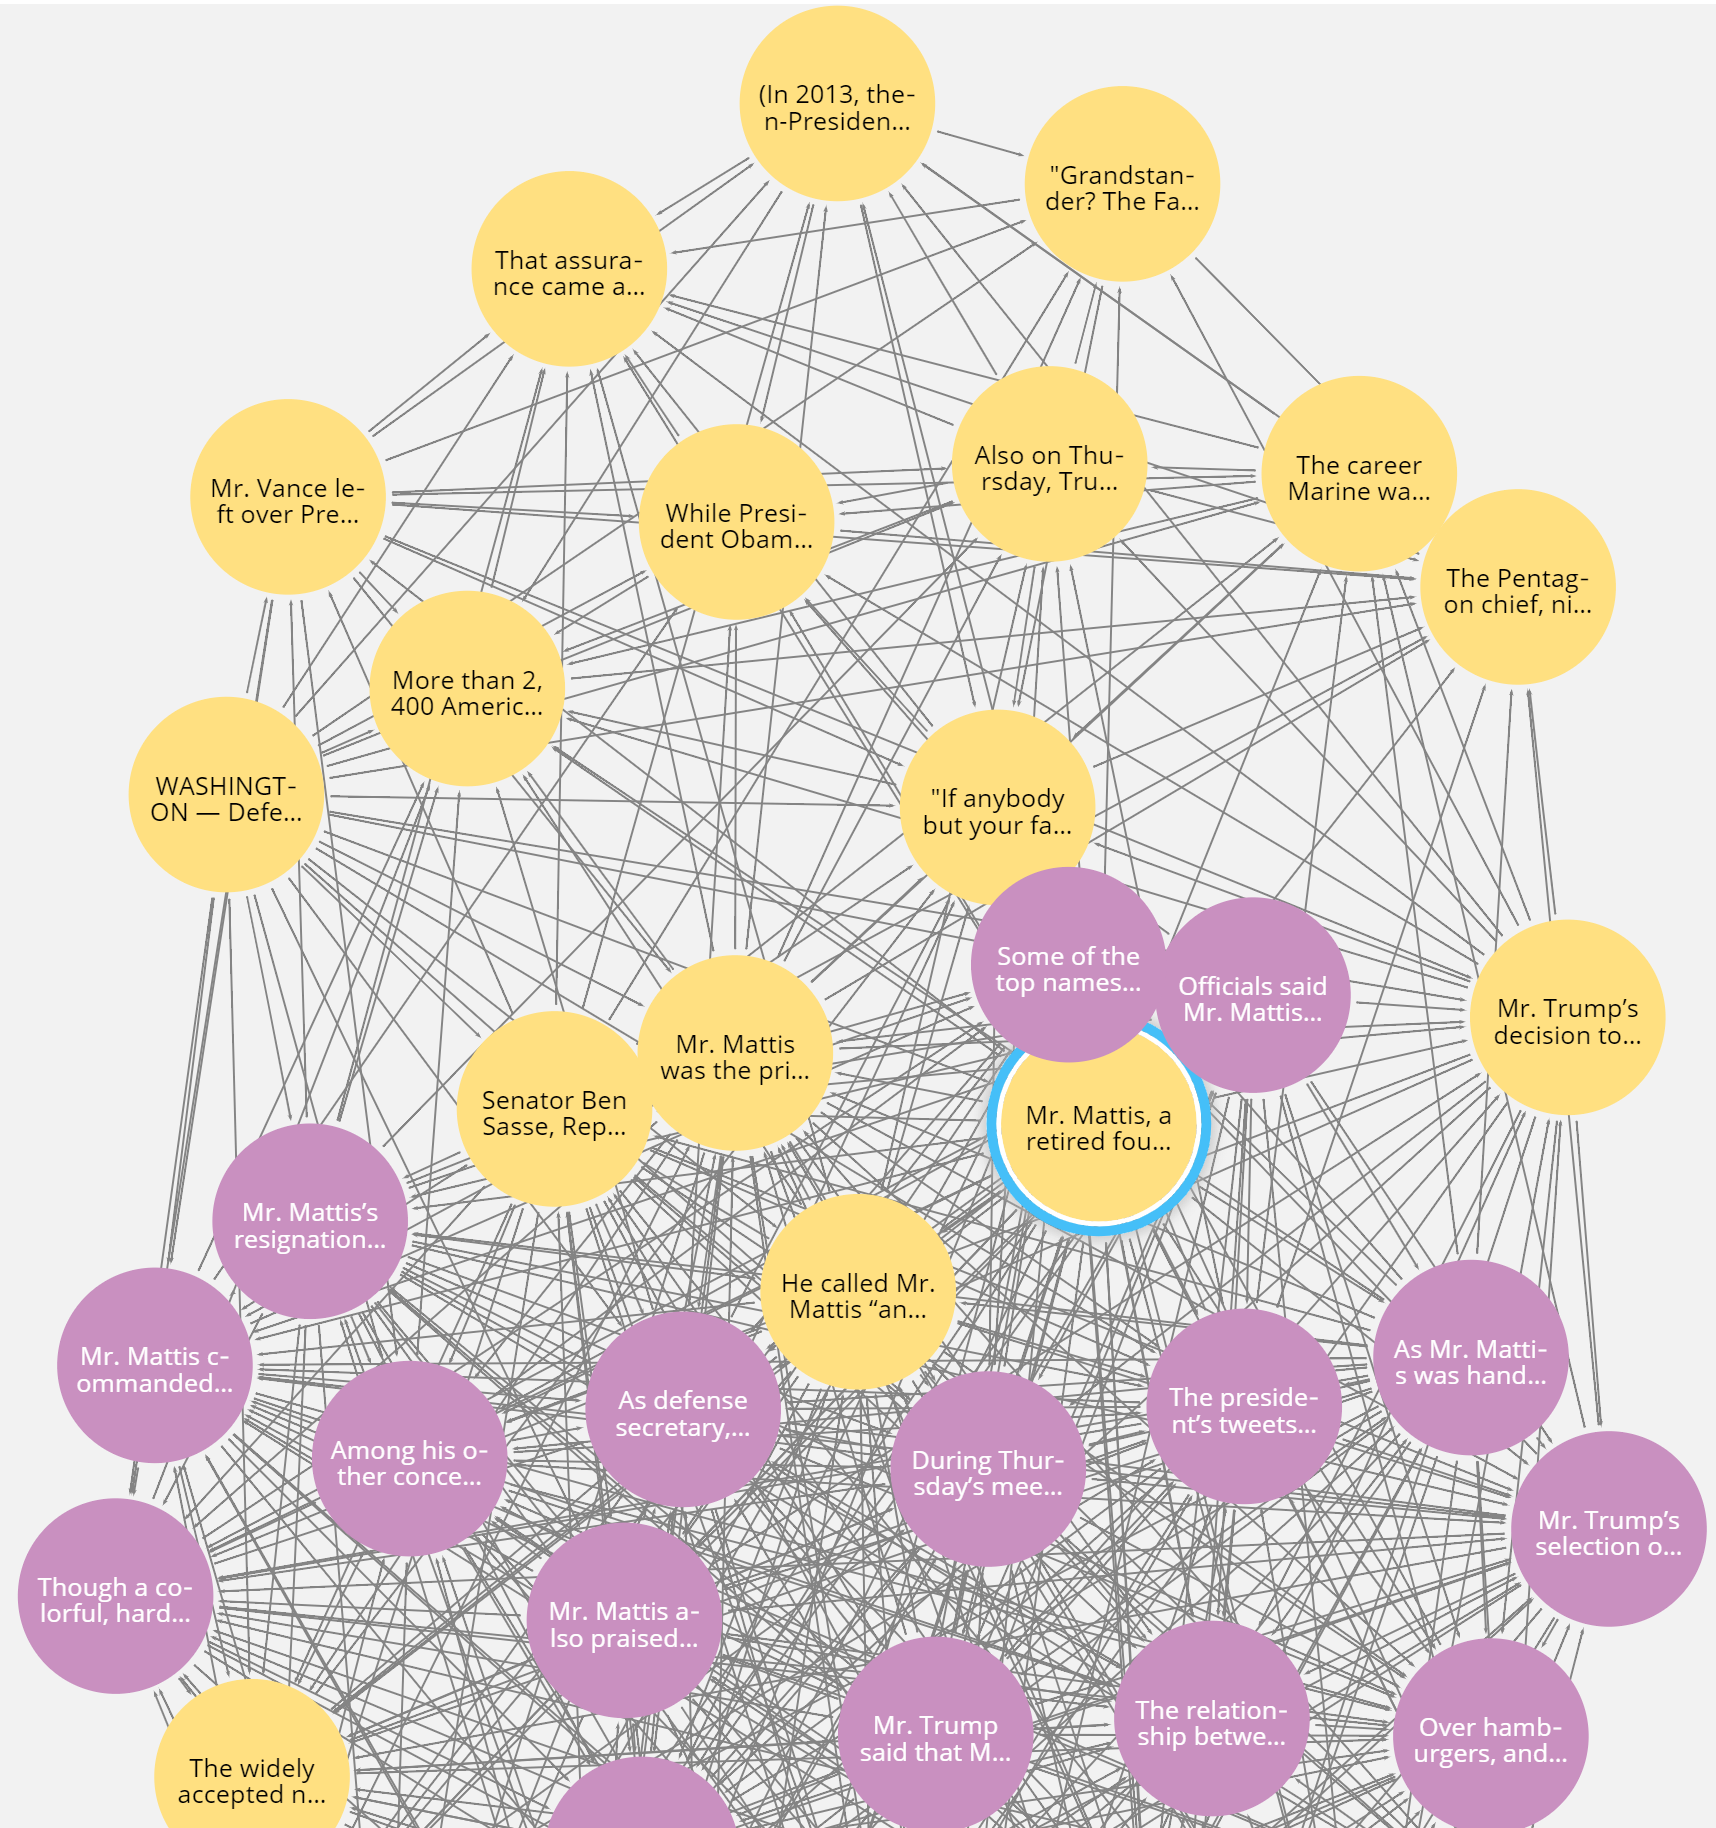
\includegraphics[]{img/mattis0_bias.png}}
    \caption{\scriptsize nodes are colored by bias label.}
    \label{subfig:mattisbias}
  \end{subfigure}
   \caption{\scriptsize Relational sentence graph} 
  \label{fig:adg}
\end{figure}



The four types of edge formation take different degrees of context into account: Type 1 and Type 2 consider only the subsequent sentences in the same article (neighborhood-context). In particular, Type 2 considers only the immediately following sentence. Type3 and Type 4 are not limited to adjacent sentences. Rather they consider the whole event (event-context). Note that edges occur only between in-event sentences, which is consistent with our event- based splitting.
% the first two types happen among only subsequent sentences in same article , especially the second one considers only the immediately following sentence; 

Figure \ref{subfig:mattissrc} and \ref{subfig:mattisbias} present the same subgraph taken directly from the real relational sentence graph in our study. We only present part of edges connected by the sentence \textit{"Mr. Mattis, a retired four-star Marine general, was rebuffed.", NYT} described in Section \ref{sent:mattis}, and the first sentence in Table \ref{tab:basil} is effectively linked to it. Moreover, nodes in Figure \ref{subfig:mattissrc} are colored according to news source (HPO/NYT/FOX) and we clearly see that relational sentence graph infuse information from different news media. In comparison of Figure \ref{subfig:mattisbias}, we found that most sentences from HPO and FOX (yellow and violet) related to target sentence are biased. Therefore event-context contained in articles of different news outlets effectively helps identify the biased sentences.

Our graph composition is intended to mimic the way humans develop views: people acquire information through immediate context in article and reason by aggregating certain background knowledge from different news reports of the whole event.

%  inspired by the Approximate Discourse Graph(ADG)
\subsection{Graph Attention Network}

As one of the representative graph convolutional networks, Graph Attention Networks (GATs) introduces an attention mechanism to achieve better neighbor aggregation. By learning the weights of the neighbors, GAT can learn the representation of the target node by implementing a weighted aggregation of the neighbor node representations. However, it may suffer from graph noise introduced by incorrect node linking. In our study, we use Self-supervised Graph Attention Network \citet{kim2021how} which introduces, on top of the GAT, an edge presence prediction task and  thus puts an emphasis on more on distinguishing misconnected neighbors.

The graph structure naturally places each sentence within its context, and as a result, different sentences are no longer isolated. The flexibility of the graph structure also allows it to move beyond the ordered arrangement of traditional LSTM. Therefore two sentences can be directly connected by edges, even if they are far apart in the original article or in different articles. 
% that are far apart in the original article or even not in the same article can be directly connected by edges. 

\KZ{One thing you need to explain is that while the relational sentence graph
contain four different edge types, these types are not distinguished here in
the GAN. Why? Would it be better to find a way to make such distinction?}

Note that our sentence graph doesn't contain edges between two events, therefore it assures no data leakage while training GAT on the whole graph.

%%%%%%%%model%%%%%%%%%%%%%%%%%%%%%%%%%%%%%%%%%%%%%%%%%%%%%%
\begin{figure*}[!htbp]\centering\scriptsize
\begin{subfigure}[t]{.2\linewidth}
  \resizebox{!}{!}{
    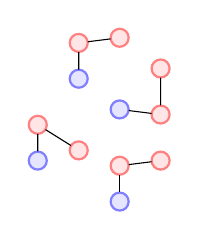
\begin{tikzpicture}[scale=.13, transform shape,
      vertex/.style = {circle, minimum width=50pt, minimum height = 17pt, draw=red!50, fill = red!10, thick},
      neg/.style = {circle, minimum width=50pt, minimum height = 17pt, draw=blue!50, fill = blue!10, thick},
      textbox/.style = {rectangle, minimum width=300pt, minimum height = 200pt},
      edge_style/.style={draw=black}]
    %   \node[event](s1) at (7,7.7) {};
    %   \node[textbox][] at (8,4) {\huge contrastive learning};
    \node[vertex] (n1) at (-8,7.5)  {};
      \node[neg] (n2) at (-8,4)  {};
      \node[vertex] (n3) at (-4,5)  {};
      
      \node[vertex] (n4) at (0,3.5)  {};
      \node[neg] (n5) at (0,0)  {};
      \node[vertex] (n6) at (4,4)  {};
      
    \node[vertex] (n7) at (-4,15.5)  {};
      \node[neg] (n8) at (-4,12)  {};
      \node[vertex] (n9) at (0,16)  {};
      
      \node[vertex] (n10) at (4,8.5)  {};
      \node[neg] (n11) at (0,9)  {};
      \node[vertex] (n12) at (4,13)  {};
      
      
      \foreach \from \to /\weight in {n1/n2/, n1/n3/, n4/n5/,n4/n6/, n7/n8/,n7/n9/, n10/n12/, n10/n11/}
        \draw[edge_style] (\from) -- node {\weight}(\to);
    \end{tikzpicture}
    \begin{tikzpicture}[scale=.7, transform shape,
      vertex/.style = {circle, minimum width=1pt, minimum height = 1pt, draw = white, fill = white},
      edge_style/.style={-stealth, draw=black, thick}]
      \node[vertex] (n1) at (-15,1.25)  {};
    %   \node[vertex] (n2) at (10, 8.5)  {};
     \node[vertex] (0) at (0,0) {};
      \node[vertex] (n3) at (-12,1.25)  {};
      \foreach \from \to /\weight in {n1/n3/}
        \draw[edge_style] (\from) -> node[above=0.1] {contrastive learning}(\to);
        \foreach \from \to /\weight in {n1/n3/}
        \draw[edge_style] (\from) -> node[below=0.1] {embedding (CSE)}(\to);
    % \foreach \from \to /\weight in {n1/n2/}
    %     \draw[edge_style,fill=white] (\from) -> node (\to);
    \end{tikzpicture}
  }
  \caption{\scriptsize triplets carefully constructed using article-based rules}
\end{subfigure}
\begin{subfigure}[t]{.3\linewidth}
  \resizebox{!}{!}{
    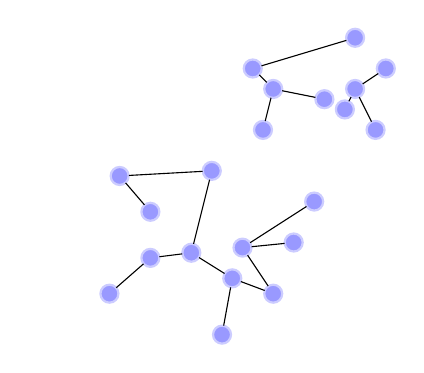
\begin{tikzpicture}[scale=.13, transform shape,
      event/.style = {rounded rectangle, minimum width=300pt, minimum height = 600pt, draw = black, fill = white, thick},
      vertex/.style = {circle, minimum width=50pt, minimum height = 50pt, draw =blue!20, fill = blue!40, thick},
      textbox/.style = {rectangle, minimum width=60pt, minimum height = 20pt},
      edge_style/.style={draw=black}]
    \node[vertex][draw=white,fill=white] (0) at (-15,0) {};
    
    \node[vertex] (n1) at (-4,7.5)  {};
      \node[vertex](n2) at (-8,4)  {};
      \node[vertex] (n3) at (0,8)  {};
      
      \node[vertex] (n4) at (4,5.5)  {};
      \node[vertex] (n5) at (3,0)  {};
      \node[vertex] (n6) at (8,4)  {};
      
    \node[vertex] (n7) at (-7,15.5)  {};
      \node[vertex] (n8) at (-4,12)  {};
      \node[vertex] (n9) at (2,16)  {};
      
    \node[vertex] (n10) at (5,8.5)  {};
      \node[vertex] (n11) at (10,9)  {};
      \node[vertex] (n12) at (12,13)  {};
      
      
        \node[vertex] (p4) at (8,24)  {};
      \node[vertex] (p5) at (13,23)  {};
      \node[vertex] (p6) at (6,26)  {};
      
    \node[vertex] (p7) at (16,24)  {};
      \node[vertex] (p8) at (15,22)  {};
      \node[vertex] (p9) at (19,26)  {};
      
    \node[vertex] (p10) at (16,29)  {};
      \node[vertex] (p11) at (18,20)  {};
      \node[vertex] (p12) at (7,20)  {};
      
    %   \node[textbox] at (4.5,1.3) {triplets};
      \foreach \from \to /\weight in {n1/n2/, n1/n3/,n3/n4/,n3/n9/, n4/n5/,n4/n6/, n7/n8/,n7/n9/, n10/n6/, n11/n10/,n12/n10/, p4/p5/,p4/p6/, p7/p8/,p7/p9/, p10/p6/, p11/p7/,p12/p4/}
        \draw[edge_style] (\from) -- node {\weight}(\to);
    \end{tikzpicture}
    % 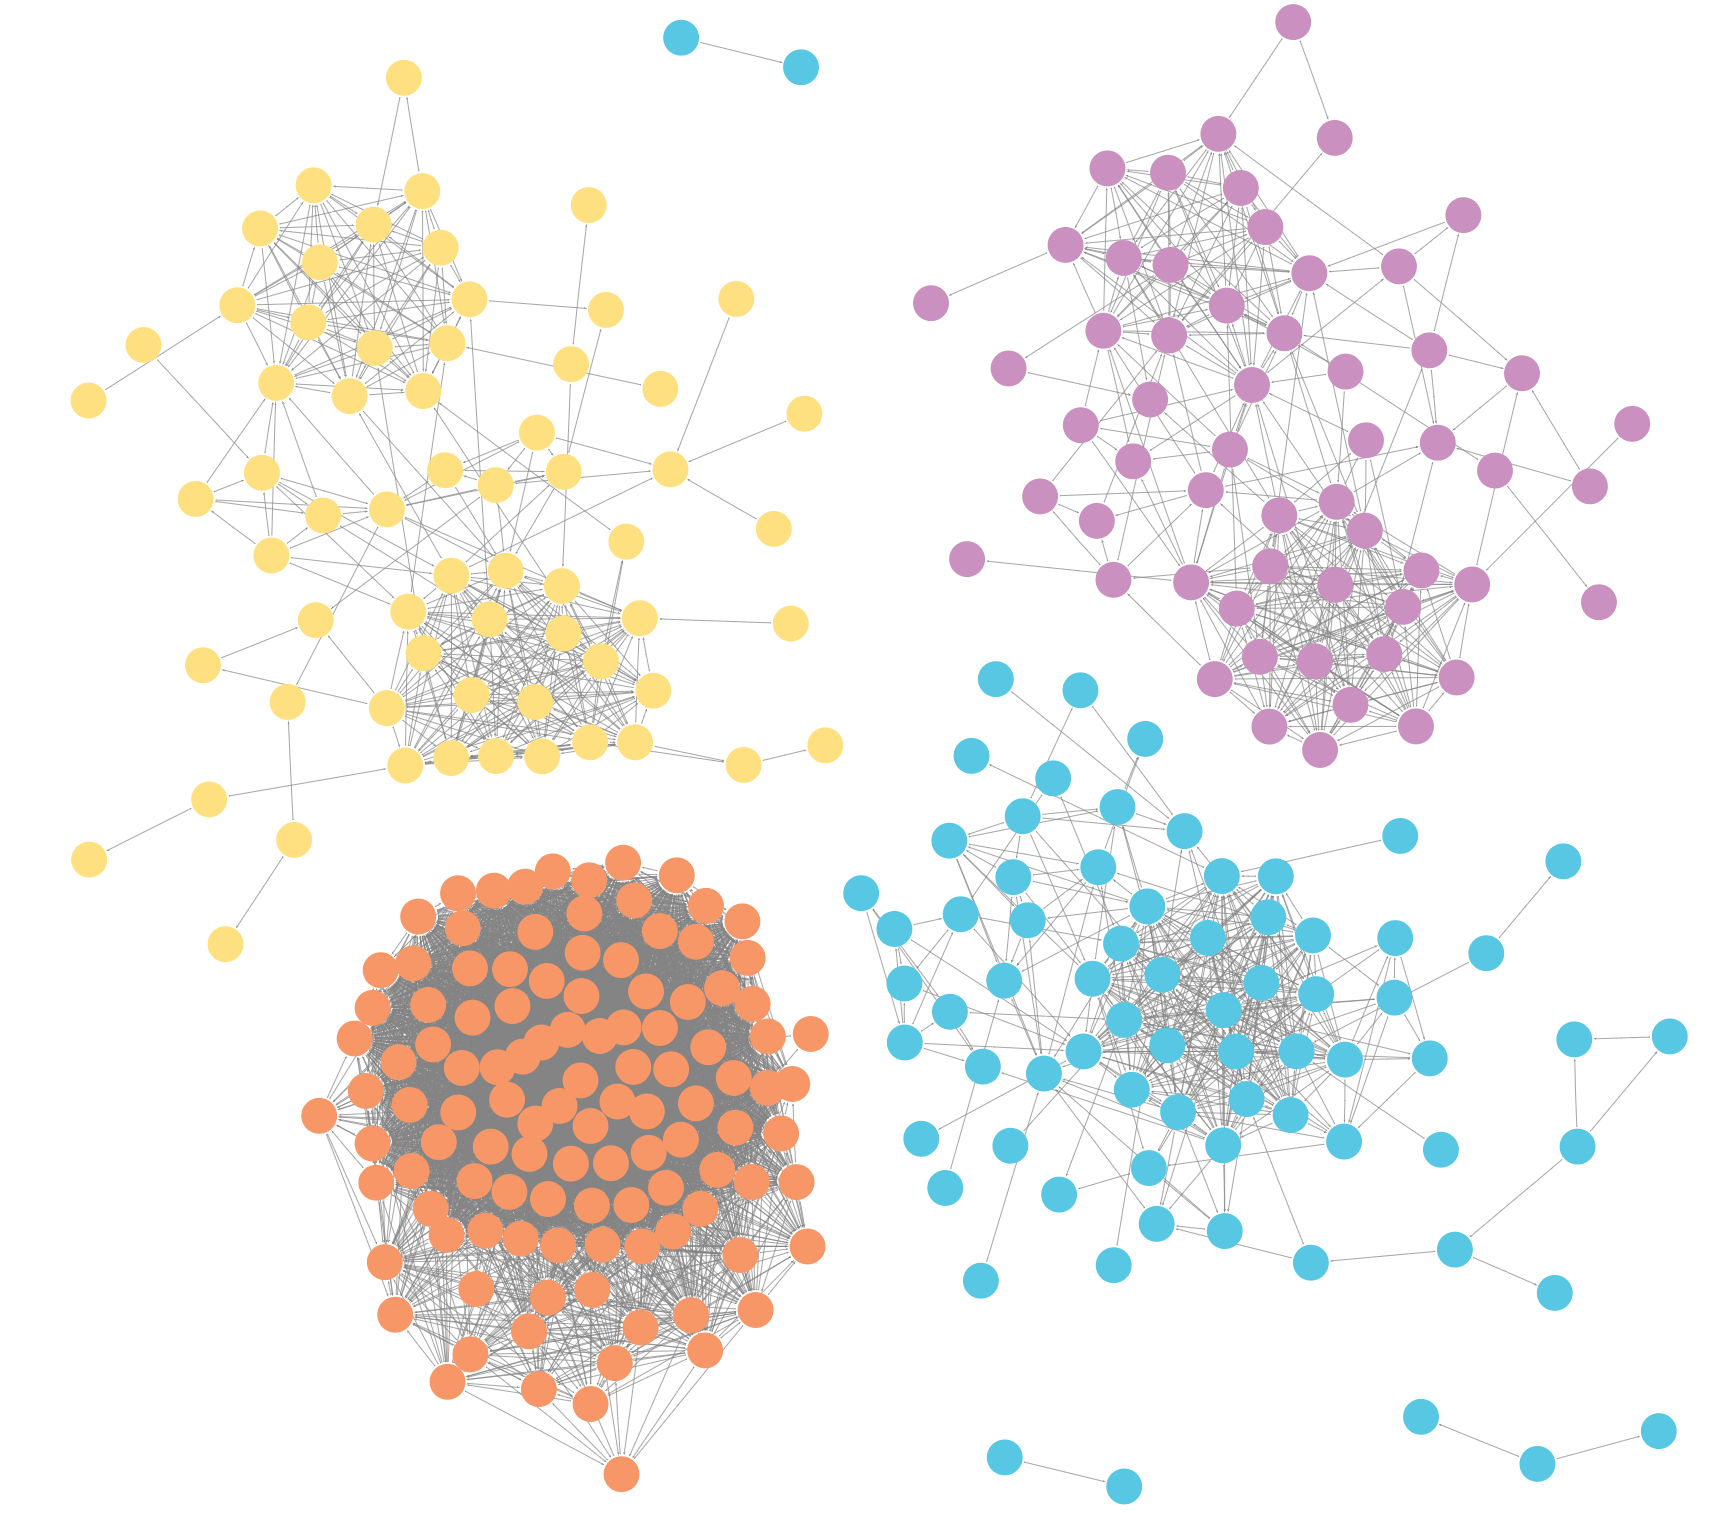
\includegraphics[]{img/sample.png}
    \begin{tikzpicture}[scale=.7, transform shape,
      vertex/.style = {circle, minimum width=1pt, minimum height = 1pt, draw = white, fill = white},
      edge_style/.style={stealth-stealth, draw=black, thick}]
      \node[vertex] (n1) at (-6,1.25)  {};
     \node[vertex] (0) at (100,0) {};
      \node[vertex] (n3) at (-3,1.25)  {};
      \foreach \from \to /\weight in {n1/n3/}
        \draw[edge_style] (\from) -> node[above=0.1] {Self-supervised }(\to);
    \foreach \from \to /\weight in {n1/n3/}
        \draw[edge_style] (\from) -> node[below=0.1] {Sentence GAT (SSGAT)}(\to);
    \end{tikzpicture}
  }
  \caption{\scriptsize Relational sentence graph: we connect two sentences if they have discourse relationships or they are semantically similar}
\end{subfigure}
\begin{subfigure}[t]{.3\linewidth}
  \resizebox{!}{!}{
    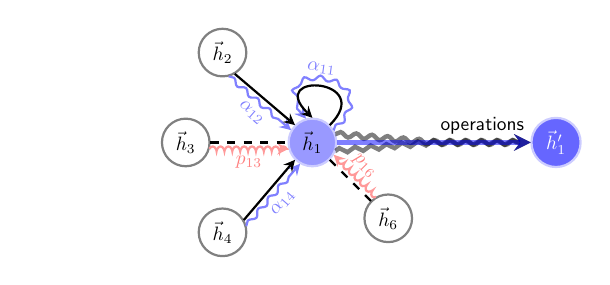
\begin{tikzpicture}[scale=.7, transform shape,
      event/.style = {rounded rectangle, minimum width=300pt, minimum height = 600pt, draw = black, fill = white, thick},
      vertex/.style = {rounded rectangle, minimum width=60pt, minimum height = 40pt, draw = black, fill = green!15, thick},
      textbox/.style = {rectangle, minimum width=60pt, minimum height = 20pt},
      edge_style/.style={draw=black, thick}]
   \node[circle] (0) at (-5,0) {};
	\node[circle, draw=blue!20, fill = blue!40, thick] (h1) {$\vec{h}_1$};
	\node[circle,draw=blue!20, fill = blue!60, thick, right=10em of h1, opacity=1] (hp) {\textcolor{white}{$\vec{h}_1'$}};
	\node[circle, draw=black!50, thick, above left=of h1] (h4) {$\vec{h}_2$};
	\node[circle, draw=black!50, thick, left=4em of h1] (h5) {$\vec{h}_3$};
	\node[circle, draw=black!50, thick, below left=of h1] (h6) {$\vec{h}_4$};
% 	\node[circle, draw, thick, below=5em of h1] (h7) {$\vec{h}_5$};
	\node[circle, draw=black!50, thick, below right=3em of h1] (h8) {$\vec{h}_6$};
	
	\draw[-stealth, red!40,thick,decoration={coil,amplitude=0.3mm,segment length=1mm}, decorate] (h8.120) -- node[sloped, above, black] {\textcolor{red!50}{$p_{16}$}} (h1.-30);
	\draw[dashed, thick] (h8.135) -- (h1.-45);
% 	\draw[-stealth, mygreen, thick, decoration={zigzag, pre length=0.01mm, segment length=2mm, amplitude=0.3mm, post length=1.5mm}, decorate] (h8.150) -- (h1.-60);
	
	\draw[-stealth, blue!50, thick,decoration={snake, pre length=0.01mm, segment length=2mm, amplitude=0.3mm, post length=1.5mm}, decorate] (h1.30) to[looseness=7] node[sloped, above, black] {\textcolor{blue!50}{${\alpha}_{11}$}}(h1.105);
	\draw[-stealth, thick] (h1.45) to[looseness=9] (h1.90);
% 	\draw[-stealth, mygreen, thick, decoration={zigzag, pre length=0.01mm, segment length=2mm, amplitude=0.3mm, post length=1.5mm}, decorate] (h1.60) to[looseness=20] (h1.75);
	
	\draw[-stealth, blue!50, thick,decoration={snake, pre length=0.01mm, segment length=2mm, amplitude=0.3mm, post length=1.5mm}, decorate] (h4.285) -- node[sloped, below, black] {\textcolor{blue!50}{${\alpha}_{12}$}}(h1.150);
	\draw[-stealth,  thick] (h4.300) -- (h1.135);
% 	\draw[-stealth, mygreen, thick, decoration={zigzag, pre length=0.01mm, segment length=2mm, amplitude=0.3mm, post length=1.5mm}, decorate] (h4.315) -- (h1.120);
	
	\draw[-stealth, red!40, thick,decoration={coil,amplitude=0.3mm,segment length=1mm}, decorate] (h5.-15) -- node[sloped, below, black] {\textcolor{red!50}{$p_{13}$}}(h1.195);
	\draw[dashed, thick] (h5.0) -- (h1.180);
% 	\draw[-stealth, mygreen, thick, decoration={zigzag, pre length=0.01mm, segment length=2mm, amplitude=0.3mm, post length=1.5mm}, decorate] (h5.15) -- (h1.165);
	
	\draw[-stealth, blue!50, thick,decoration={snake, pre length=0.01mm, segment length=2mm, amplitude=0.3mm, post length=1.5mm}, decorate] (h6.15) -- node[sloped, below, black] {\textcolor{blue!50}{${\alpha}_{14}$}}(h1.240);
	\draw[-stealth, thick] (h6.30) -- (h1.225);
% 	\draw[-stealth, mygreen, thick, decoration={zigzag, pre length=0.01mm, segment length=2mm, amplitude=0.3mm, post length=1.5mm}, decorate] (h6.45) -- (h1.210);
	
% 	\draw[-stealth, mymauve, thick,decoration={snake, pre length=0.01mm, segment length=2mm, amplitude=0.3mm, post length=1.5mm}, decorate] (h7.75) -- node[sloped, below, black] {$\vec{\alpha}_{15}$}(h1.-75);
% 	\draw[-stealth, dashed, thick] (h7.90) -- (h1.-90);
% 	\draw[-stealth, mygreen, thick, decoration={zigzag, pre length=0.01mm, segment length=2mm, amplitude=0.3mm, post length=1.5mm}, decorate] (h7.105) -- (h1.-105);
	

	
	\coordinate[right=5em of h1] (A);
	
	\draw[-stealth,  opacity=0.5, ultra thick,decoration={snake, pre length=0.01mm, segment length=2mm, amplitude=0.3mm, post length=1.5mm}, decorate] (h1.20) -- (A) -- (hp);
	\draw[-stealth, opacity=0.5, ultra thick,decoration={zigzag, pre length=0.01mm, segment length=2mm, amplitude=0.3mm, post length=1.5mm}, decorate] (h1.-20) -- (A) -- (hp);
	\draw[-stealth, blue, opacity=0.5, ultra thick] (h1.0) -- (A) -- node[black, above, opacity=1.0] {operations} (hp);
    \end{tikzpicture}
  }
    \caption{\scriptsize Self-supervised GAT, where \textcolor{blue!60}{$\alpha_{ij}$} denotes attention between node $i$ and $j$, \textcolor{red!60}{$p_{ij}$} denotes the probability of the presence of edge between node $i$ and $j$}
\end{subfigure}
  \caption{ Our Model MultiCTX }
  \label{fig:model}
\end{figure*}

% \KZ{The boundaries between the subfigures are not clear.}



% In short, our model places individual sentences within a broader contextual background knowledge and model is able to understand them through direct information transfer via edges.


\section{Experiment and Results}

We experiment with four baselines including the current state-of-the-art model and four variants of MultiCTX in order to fully demonstrate each module's utility. Our results suggest that MultiCTX greatly outperforms the current SOTA and effectively incorporates the contextual information in sentence-level informational bias detection.

\subsection{Set-up}

We use the same 10-fold cross-validation event-split in \citet{van-den-berg-markert-2020-context} to facilitate the comparison.

Each fold has 80/10/10 non-overlapping events for train/val/test partition, and sentences from the same event never appear simultaneously in two different subsets within one fold. There are on average 6400/780/790 sentences in train/val/test set respectively. We use 5 different seeds for each method and the F1 score, precision and recall ('biased' is positive class) as the evaluation metrics. For each experiment, a mean value and standard deviation across 5 seeds will be reported if applicable.

We use the same hyper-parameters provided in \citep{van-den-berg-markert-2020-context} to reimplement BERT, RoBERTa and WinSSC baselines. However, for EvCIM, We cut the training epochs from 150 to 75 and increase the batch size from 32 to 64 due to the considerable time usage. For MultiCTX, We trained  use a RoBERTa-based contrastive learning following the implementation in \citep{gao2021simcse}. Due to unavoidable non-deterministic atomic operations in implementation of GAT, the result presented below may cannot be exactly reproduced, but we took an average on our experiments to reflect its range. All models are trained and evaluated on a GeForce GTX 1080 Ti GPU with 11G RAM and Intel(R) Xeon(R) CPU E5-2630 with 128G of RAM. Training details will be described in Appendix.

% For MultiCTX, We use epochs=5, max length=256, lr = 4.5e-5, training batch size=16 in RoBERTa-based contrastive learning following the implementation in \citep{gao2021simcse}. We use adjacent sentence limitation = 5, semantic similarity threshold=0.98 in the construction of relational sentence graphs. Due to unavoidable non-deterministic atomic operations in implementation of GAT, the result presented below may cannot be exactly reproduced, but we took an average on our experiments to reflect its range. We use a one-layer SuperGAT with heads=1, negative sample ratio = 0.9, dropout = 0.1, learning rate = 0.1, l2 regularization = 1e-4, attentional loss weight = 1e-3 and then train for 300 epochs to select the best result.All models are trained and evaluated on a GeForce GTX 1080 Ti GPU with 11G RAM and Intel(R) Xeon(R) CPU E5-2630 with 128G of RAM.


\subsection{Baselines}

There are few models in sentence-level informational bias detection. \citet{fan-etal-2019-plain} has proposed BASIL dataset and corresponding BERT and RoBERTa benchmarks. \citet{cohan-etal-2019-pretrained} has proposed several models trying to incorporate context in different ways. We will take two of them, WinSSC and their best and also current SOTA model EvCIM, as our baselines. Few other works used BASIL dataset but with objectives other than sentence-level informational detection. Thus we have four baseline models:

\begin{itemize}
    \item \textbf{BERT} \citep{devlin-etal-2019-bert} and \textbf{RoBERTa} \citep{liu2019roberta}: we finetune the individual sentence informational bias detection task on $\text{BERT}_{base}$ and $\text{RoBERTa}_{base}$.
    \item \textbf{WinSSC} \citep{van-den-berg-markert-2020-context}
        
        WinSSC (windowed Sequential Sentence Classification) is a variant of SSC \citep{cohan-etal-2019-pretrained}. We include it as one of the baselines because SSC implements the very natural idea that comes to us when we think of using context: directly inputing sequences of consecutive sentences to BERT. SSC feeds the concatenation of sentences from a chunk of document to pretrained language models (PLMs),and  then classifies each sentence using the embedding of the separator tokens \texttt{[SEP]} at its end. SSC makes non-overlapping chunks while WinSSC makes chunks by overlapping sentences at both ends, which eretains the contextual information for bookended sentences. 
        
    \item \textbf{EvCIM}\label{para:evcim}  : PLM embeddings + BiLSTM
    
        EvCIM (Event Context-Inclusive Model) proposed by \citet{cohan-etal-2019-pretrained} is the SOTA model on BASIL dataset and it also uses the contextual information.
         It takes the average of the last four layers of fine-tuned $\text{RoBERTa}_{base}$ as the sentence embedding, and then uses BiLSTM to encode each article from the same event as the target sentence. Finally it concatenates three article representations and the target sentence embedding to make the sentence-level prediction. Besides using the hyper-parameters from the original paper, we generate the result from a separate set of reasonable hyper parameters. We present below results both from the original paper and from our experiments.
        %  We reproduce it in our study using other reasonable hyper-parameters different with the original version. and will show both results from the original paper and from our experiments.
    
\end{itemize}



\subsection{Our Models}
\begin{itemize}
    \item \textbf{CSE: Contrastive Sentence Embedding}
    
    Classification by a logistic regression on sentence embeddings directly obtained from contrastive learning.
    
    \item \textbf{EvCIM w/ CSE}: CSE + BiLSTM
    
    Similar to EvCIM described in Section \ref{para:evcim}, we utilize BiLSTM-encoded context as well as the target sentence to perform the sentence-wise classification. However, instead of the average of the last four layers of fine-tuned $\text{RoBERTa}_{base}$ in EvCIM, we use CSE (Contrastive Sentence Embedding) in our study. Moreover, we also add news source embeddings before the final fully connected classification layer on top of BiLSTM-encoded in-event article embeddings. 
    
    In the original paper \citep{cohan-etal-2019-pretrained}, adding news source embeddings hurts EvCIM's performance, but because it is useful for EvCIM w/ CSE according to our experiments, we use this version here. This also indicates that CSE has better captured inherent properties of sentences compared to PLM embeddings. CSE can therefore well incorporate extra news media information rather than be disturbed by it.
    
    \item \textbf{MultiCTX w/o CSE}: PLM embeddings + SSGAT
    
    We use the original sentence embedding in EvCIM, which is the
    the average of the last four layers of fine-tuned $\text{RoBERTa}_{base}$ to build the relational sentence graph. We then apply Self-supervised GAT on the graph (SSGAT, Self-supervised Sentence GAT). In other words, we replace CSE in MultiCTX with EvCIM's sentence embedding.
    
    \item \textbf{MultiCTX}: our full model (CSE + SSGAT)
    
    MultiCTX first performs contrastive learning on carefully composed triplets to obtain CSE. It then builds relational sentence graph according to inter-sentence relationships. Finally, MultiCTX applies Self-supervised GAT above to get the final sentence informational bias prediction.
    
    
\end{itemize}



\begin{table*}[htbp]
  \centering \scriptsize
    \begin{tabular}{l|l|cccc}
    \toprule[1pt]
     \multicolumn{2}{c}{ \textbf{Model$^{*}$}} & \textbf{Explanation} & \textbf{Precision} & \textbf{Recall} & \textbf{F1} \\
    \midrule
    % BERT in \citet{van-den-berg-markert-2020-context}   & 38.96 \pm 5.55 & 35.79\pm2.15& 37.00\pm 2.11 \\
    % \hline
    % RoBERTa in \citet{van-den-berg-markert-2020-context} & 43.12\pm1.03 & 41.29 \pm 1.37    & 42.16 \pm 0.30 \\
    % \hline
    % WinSSC in \citet{van-den-berg-markert-2020-context} & 42.28 \pm0.99& 36.94\pm 0.88  & 38.67 \pm 0.82 \\
    \multirow{5}{*}{baselines} & $\text{BERT}_{base}$  &  & $40.44 \pm 1.07^{**}$ & $31.65\pm1.11$& $35.49\pm 0.67$ \\ \cline{2-6}
    &$\text{RoBERTa}_{base}$ & & $44.588\pm0.80$ & $40.02 \pm 2.22$    & $42.13 \pm 1.02$ \\  \cline{2-6}
    &WinSSC & &$41.47\pm1.31$& $34.37\pm 0.57$  & $37.58 \pm 0.77$ \\ \cline{2-6}
    &EvCIM (our reproduction)
     &  \multirow{2}{*}{PLM embed. + BiLSTM} & $38.40 \pm 0.64$   & $48.53\pm 1.45$& $42.87 \pm 0.69$ \\
    &EvCIM (original paper)
      &  & $39.72\pm 0.59$ &  $49.60 \pm 1.20$ & $44.10\pm 0.15$ \\ \hline
    \multirow{4}{1cm}{models}&CSE   &  & 47.53     & 40.13     & 43.51  \\ \cline{2-6}
    &EvCIM w/ CSE & CSE+BiLSTM &$48.53 \pm 0.73$     & $41.98\pm 0.36$    & $45.01 \pm 0.26$\\ \cline{2-6}
    &MultiCTX w/o CSE & PLM embed.+ SSGAT &   $46.89 \pm 0.71$  &  $42.88\pm 0.67$   & $44.79 \pm 0.63$ \\ \cline{2-6}
    &MultiCTX (full) & CSE+SSGAT &  $47.78 \pm 0.94$   &  $44.50 \pm 0.65$   & $\mathbf{46.08 \pm 0.21}^{***}$ \\
    \bottomrule[1pt]
    \multicolumn{5}{l}{$^{*}$ \scriptsize All results are implemented or reproduced by ourselves except for the second EvCIM record} &\\
    \multicolumn{5}{l}{$^{**}$  \scriptsize Mean value and standard deviation across 5 seeds are reported if applicable} & \\
    \multicolumn{6}{l}{$^{***}$  \scriptsize The best result on a single run obtained in our experiments is \textbf{F1=46.74}} \\
    % Due to unavoidable non-deterministic atomic operations in implementation, the result here may cannot be reproduced exactly, but we took an average on our experiments to reflect its range. Also 

    \end{tabular}%
  \caption{ Results}
  \label{tab:res}%
\end{table*}%


\paragraph{1. Encoding sequential sentences brutally by PLM may fail.}

Here we use $\text{RoBERTa}_{base}$ as pretrained language model in WinSSC. However, it obtains worse result (F1=37.58) than the original $\text{RoBERTa}_{base}$ (42.13). The result is similar as in \citet{van-den-berg-markert-2020-context}. There are two possible reasons: First, we take sentence chunks instead of individual sentences as input, and doing so may introduce data reduction. Second, BERT-based pretrained language models are not good at processing long text. They simply join neighboring sentences, which may introduce more noise and complexity rather than help integrate the context. Therefore, brute-force concatenation of sequential sentences can rarely make use of the contextual information, and it probably brings in more noise and reduces the data quantity. 
%  and it may suffer from data reduction

\paragraph{2. Contrastive learning helps improve sentence embeddings.} 

The results show that contrasive sentence embeddings (CSE) classified simply with a logistic regression (F1=43.51) beats our reproduction of EvCIM (F1=42.87); moreover, CSE combined with BiLSTM (EvCIM w/ CSE, F1=45.01) outperforms EvCIM even more in comparison with the declared F1=44.10 in its original paper \citep{cohan-etal-2019-pretrained}. 

Note that EvCIM uses the average of the last four layers of fine-tuned $\text{RoBERTa}_{base}$ as the sentence embedding. Therefore, our results prove that contrastive learning produces better sentence representations than BERT-based PLMs. this can be achieved via contextual information incorporation. 

\begin{itemize}
    \item BERT-based PLM tends to encode all sentences into a smaller spatial region, which results in a high similarity score for most of the sentence pairs, even for those that are semantically completely unrelated. Specifically, when the sentence embeddings are computed by averaging the word vectors, they are easily dominated by high-frequency words, making it difficult to reflect their original semantics.
    \item Instead of individual sentences, CSE considers for each target sentence a context built up by all its positive and negative counterparts in related triplets. Among them, negative samples provide an article-level context and positive samples provide an event-level context. With the goal of contrastive learning to "distill essence", it learns from its context and naturally suppresses such shallow high-frequency-words features, thus avoiding similar representations of semantically different sentences. 
\end{itemize}



% Although the BERT-based model achieves good performance on many NLP tasks, its own derived sentence vectors are of unsatisfactory quality. 


\paragraph{3. Sentence graph can effectively integrate context.} 

We can see that MultiCTX w/o CSE, i.e. PLM embed.+SSGAT (F1=44.79) outperforms EvCIM (F1=44.10 in original paper and F1=42.87 from our reproduction). The two models both use averaged RoBERTa embedding as sentence embeddings. The former uses graph structure (SSGAT) while the latter use BiLSTMs to carry out classification. 

The results prove that our sentence graph structure is better in encoding contextual information than sequential models such as BiLSTM. We will examine different levels of context, i.e., adjacent sentences, the article and the the event context in the ablation study in the next section.


\paragraph{4. Contrastive learning together with sentence graph achieves the best performance} 

Our full model MultiCTX achieves F1=46.08 in the sentence-level informational bias detection task, significantly outperforms the current State-of-the-Art model EvCIM \citep{cohan-etal-2019-pretrained} (F1=44.10 declared in original paper). Possible reasons are: 1) BiLSTMs are limited to the event context in EvCIM; 2) MultiCTX uses better sentence representations (CSE); 3) MultiCTX incorporates the context in varying degrees explicitly using graph structure and implicitly via contrastive learning.


\section{Ablation Analysis}

% In this section we will further explore the different levels of context (adjacent sentences, article context, event context) in our model, specifically in our SSGAT. We keep CSEs fixed and modify our relational sentence graph by removing certain types of edges then report the results to see which levels of context are most important in our informational bias detection task.

We have proved that both CSE and SSGAT are essential for MultiCTX, and in this section, we will further explore roles of different inter-sentence relationships in our model. We keep CSEs fixed and modify our relational sentence graph by removing certain types of edges, and then report the results to see how each part contributes to MultiCTX in our informational bias detection task.

Edge types described in Section \ref{para:edge} can be briefly summarized in two categories: Type 1,2 and 3 are discourse relationships and Type 4 is semantic similarity. Besides, they can also be partitioned by level of context: Type 1 and 2 are neighborhood-level and article-level; Type 3 and 4 are event-level. we will focus on their utility in our ablation study. 

\begin{figure*}[!htbp]\centering
  \begin{subfigure}[t]{.15\linewidth}
    \resizebox{\linewidth}{!}{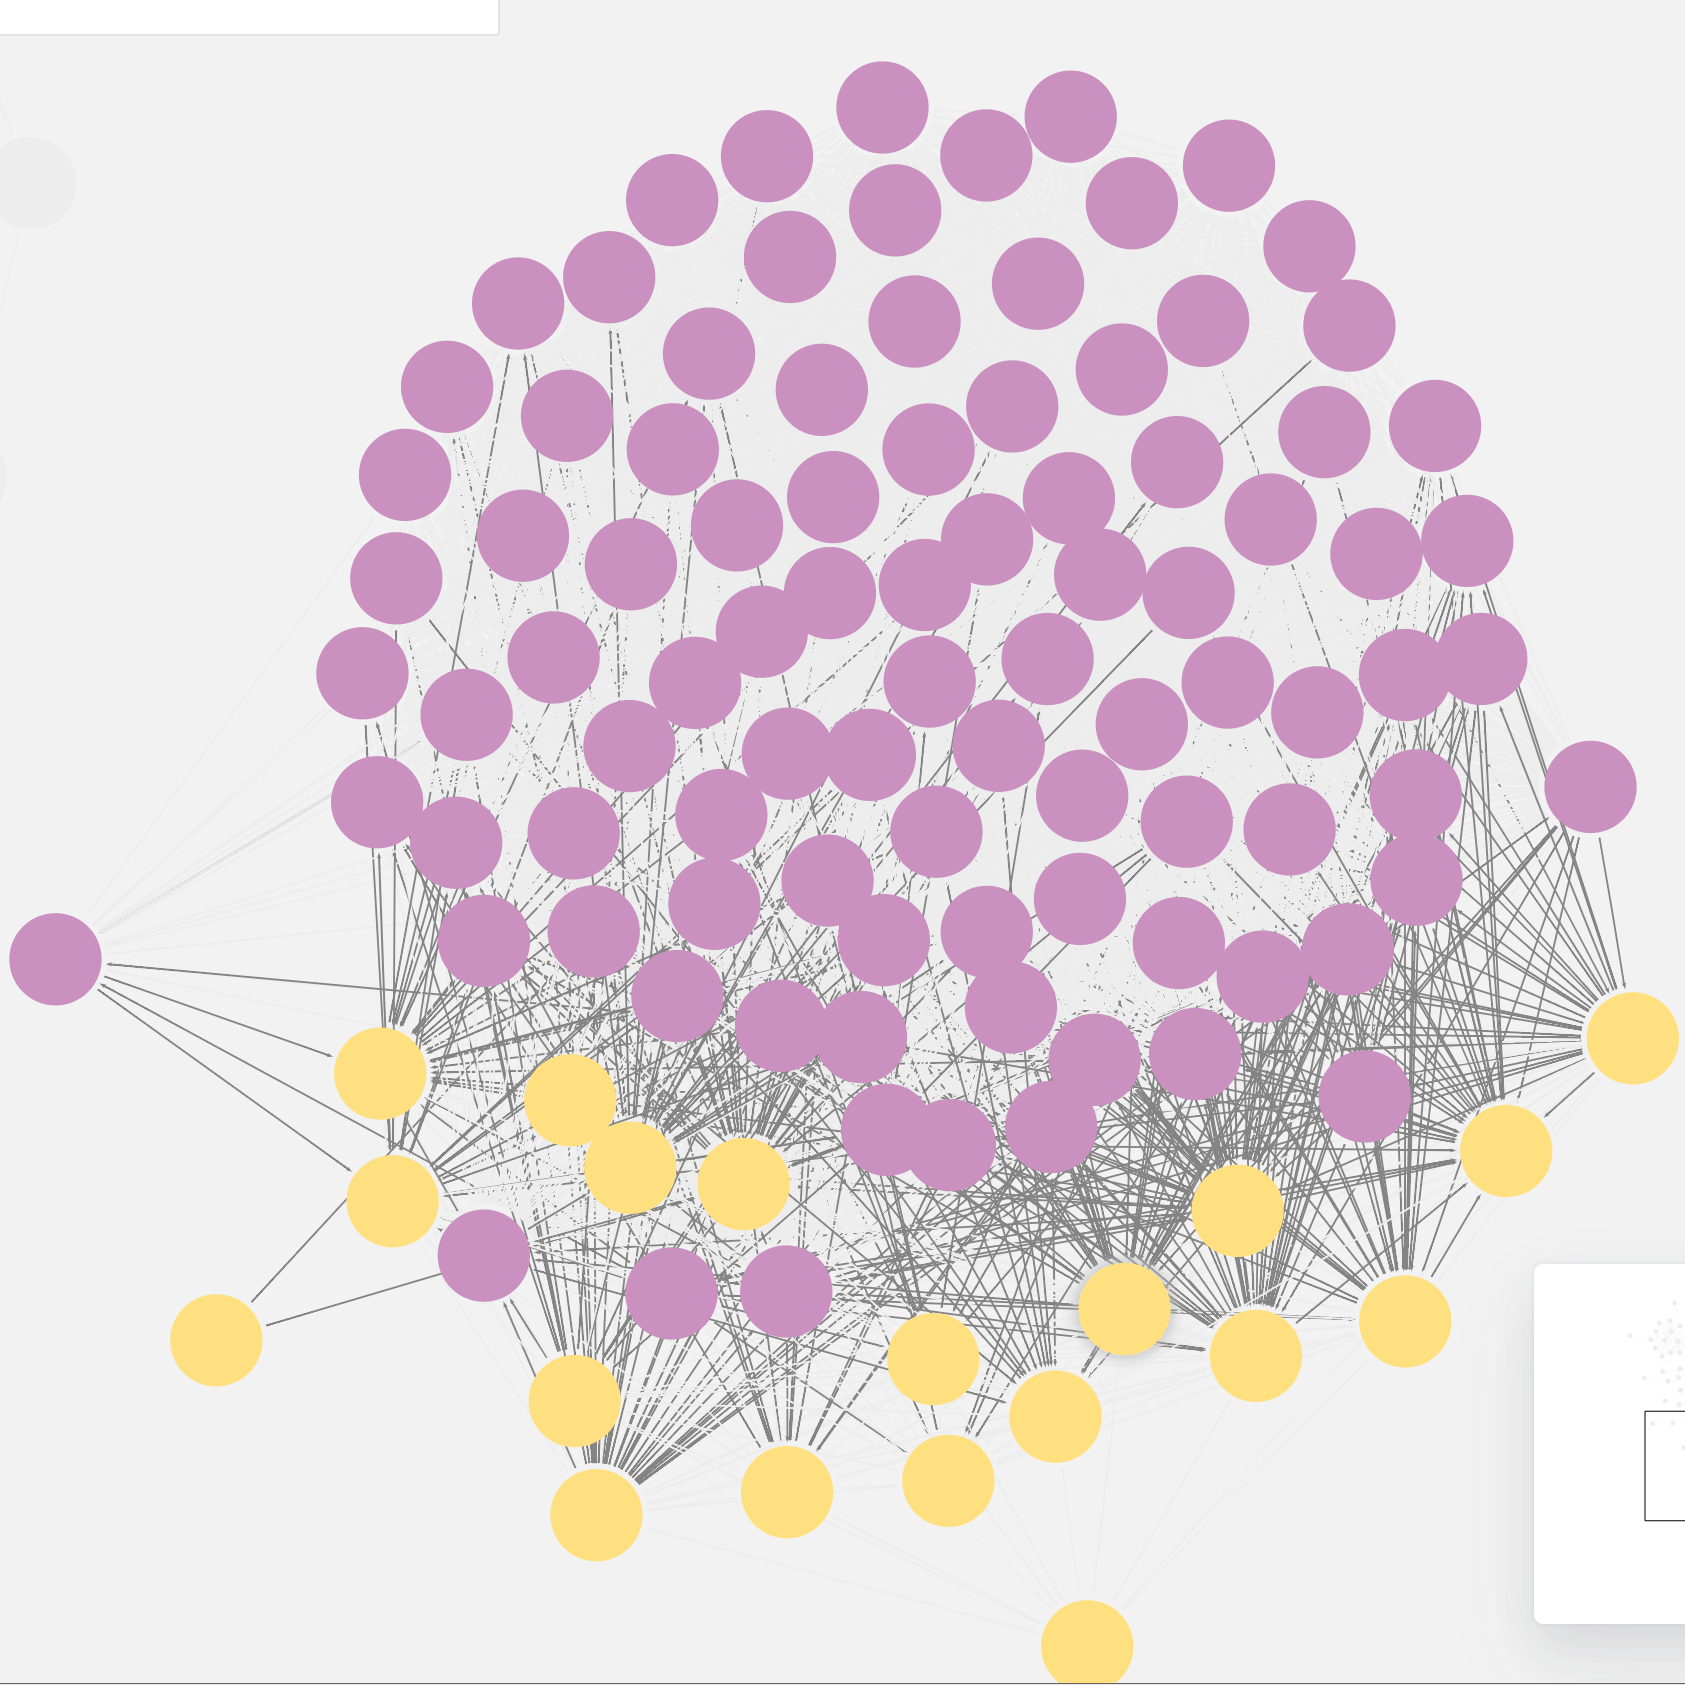
\includegraphics[]{img/only123.png}}
    \caption{\scriptsize Graph with edges of Type 1,2,3}
    \label{subfig:ab123}
  \end{subfigure}
  \begin{subfigure}[t]{.15\linewidth}
    \resizebox{\linewidth}{!}{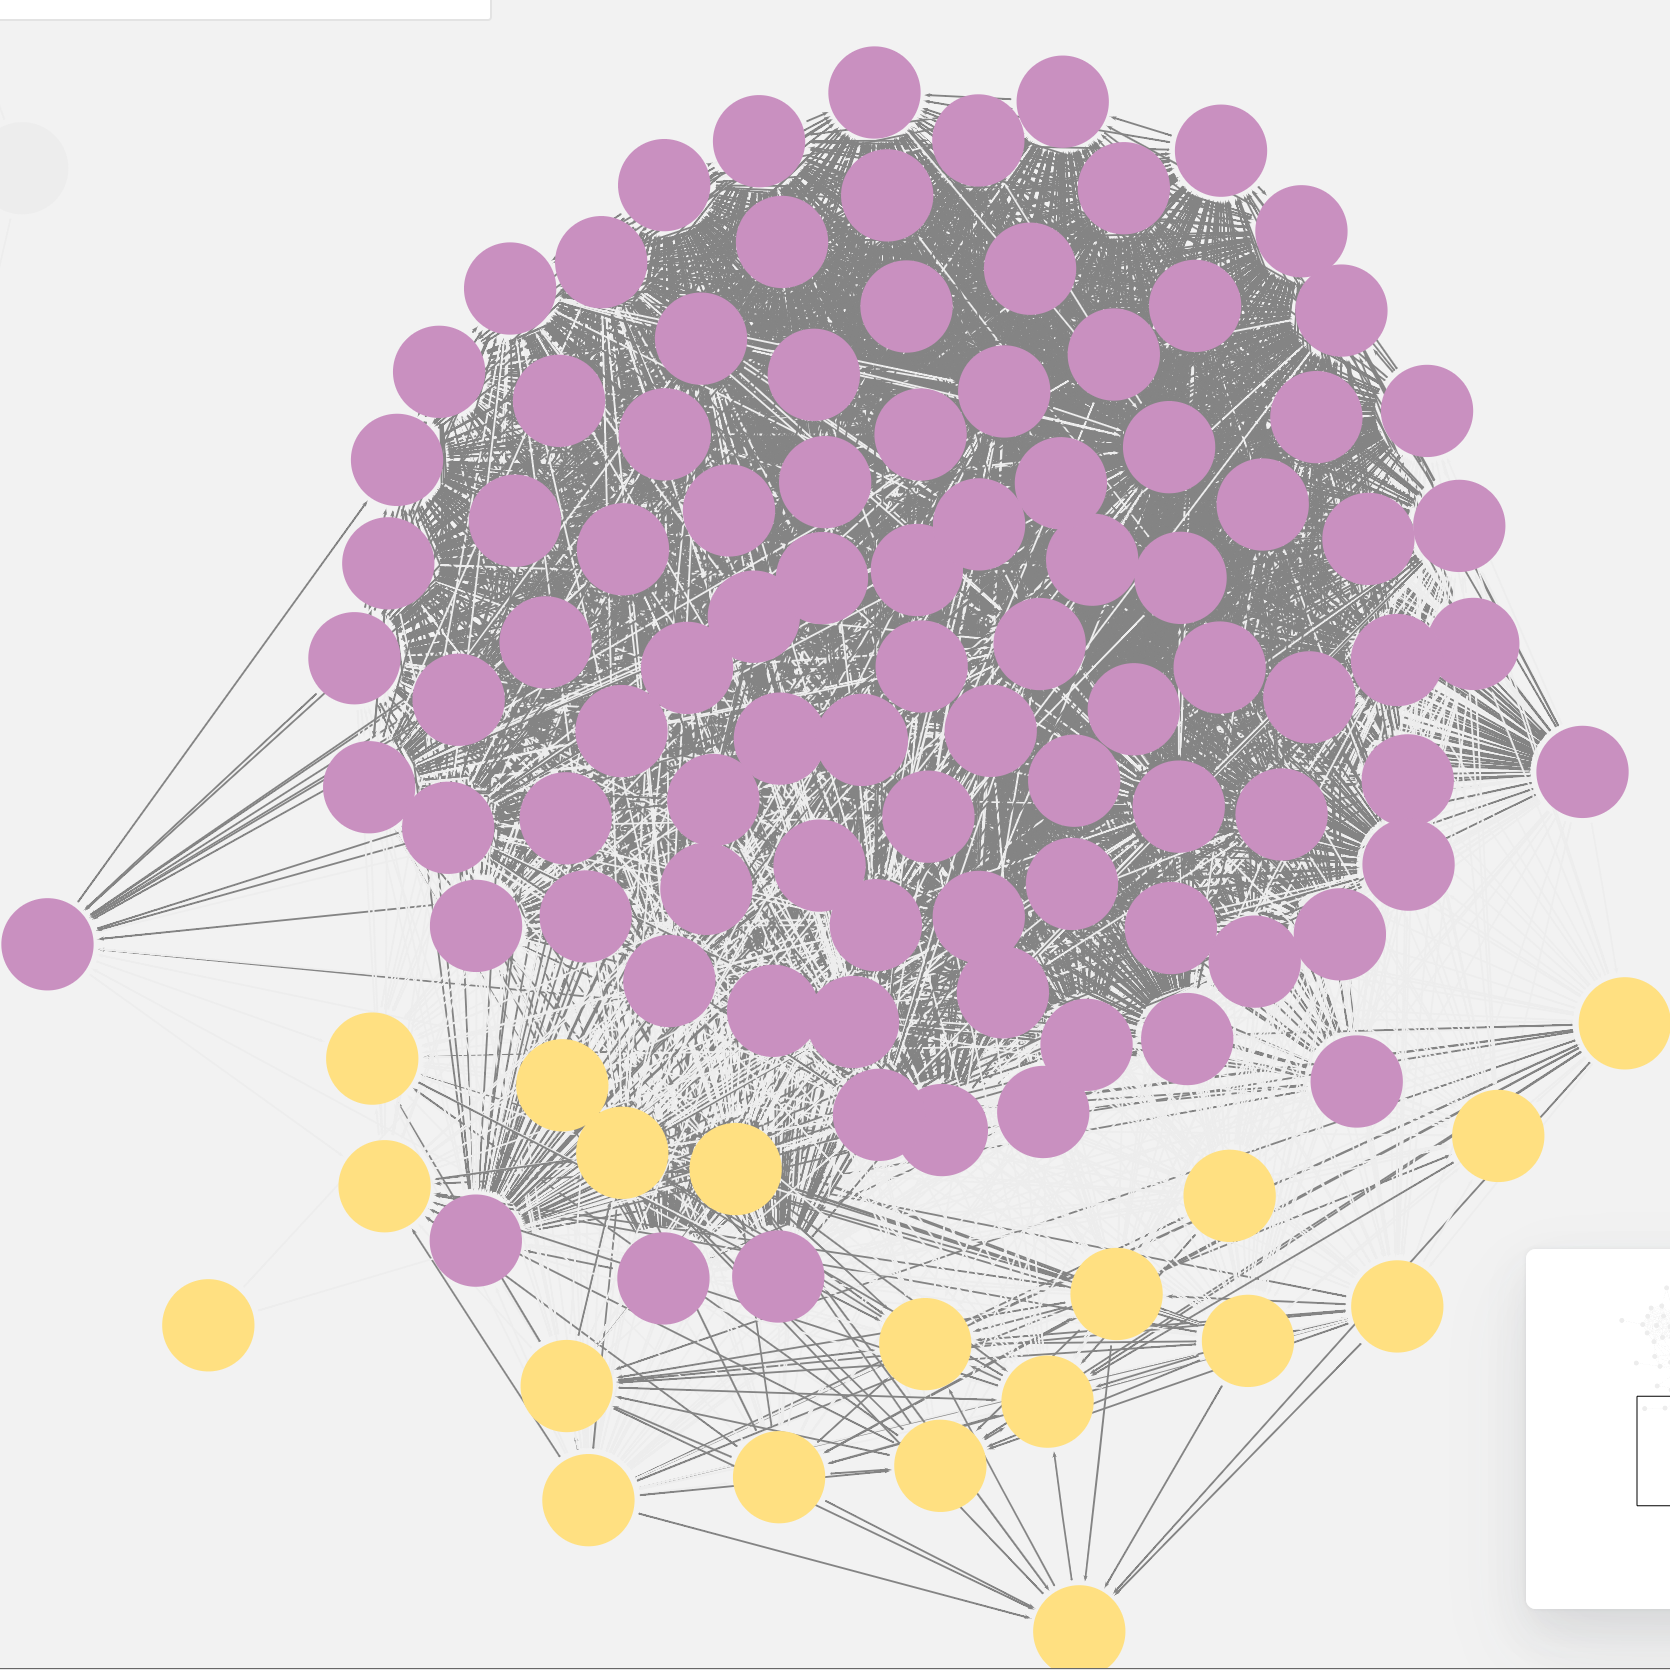
\includegraphics[]{img/only4.png}}
    \caption{\scriptsize Graph with edges of Type 4}
    \label{subfig:ab4}
  \end{subfigure}
  \begin{subfigure}[t]{.15\linewidth}
    \resizebox{\linewidth}{!}{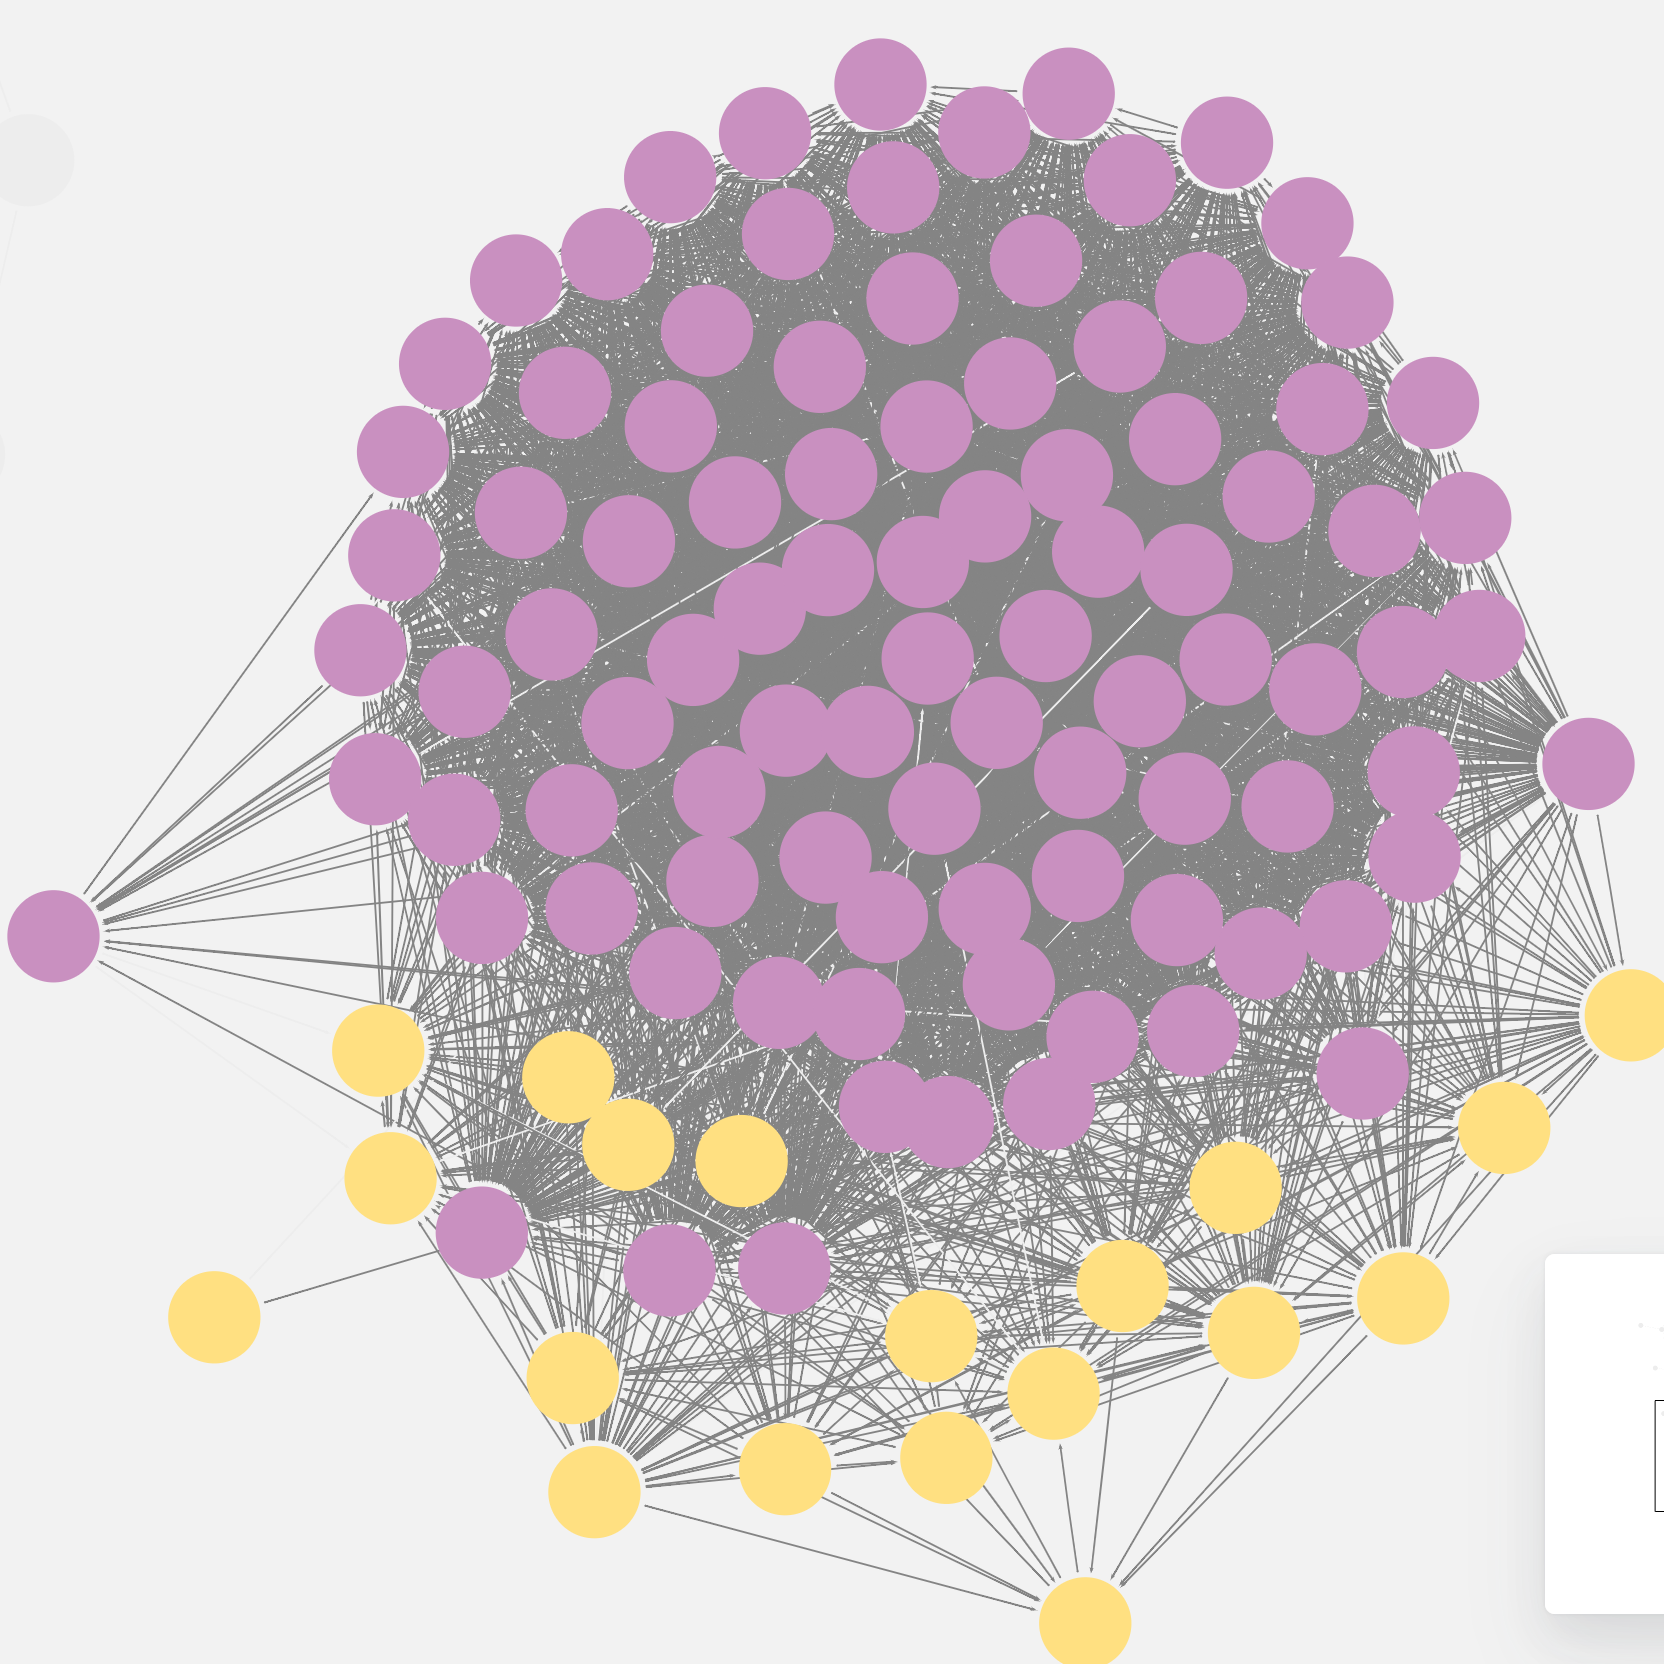
\includegraphics[]{img/only34.png}}
    \caption{\scriptsize Graph with edges of Type 3,4}
    \label{subfig:ab34}
  \end{subfigure}
  \begin{subfigure}[t]{.15\linewidth}
    \resizebox{\linewidth}{!}{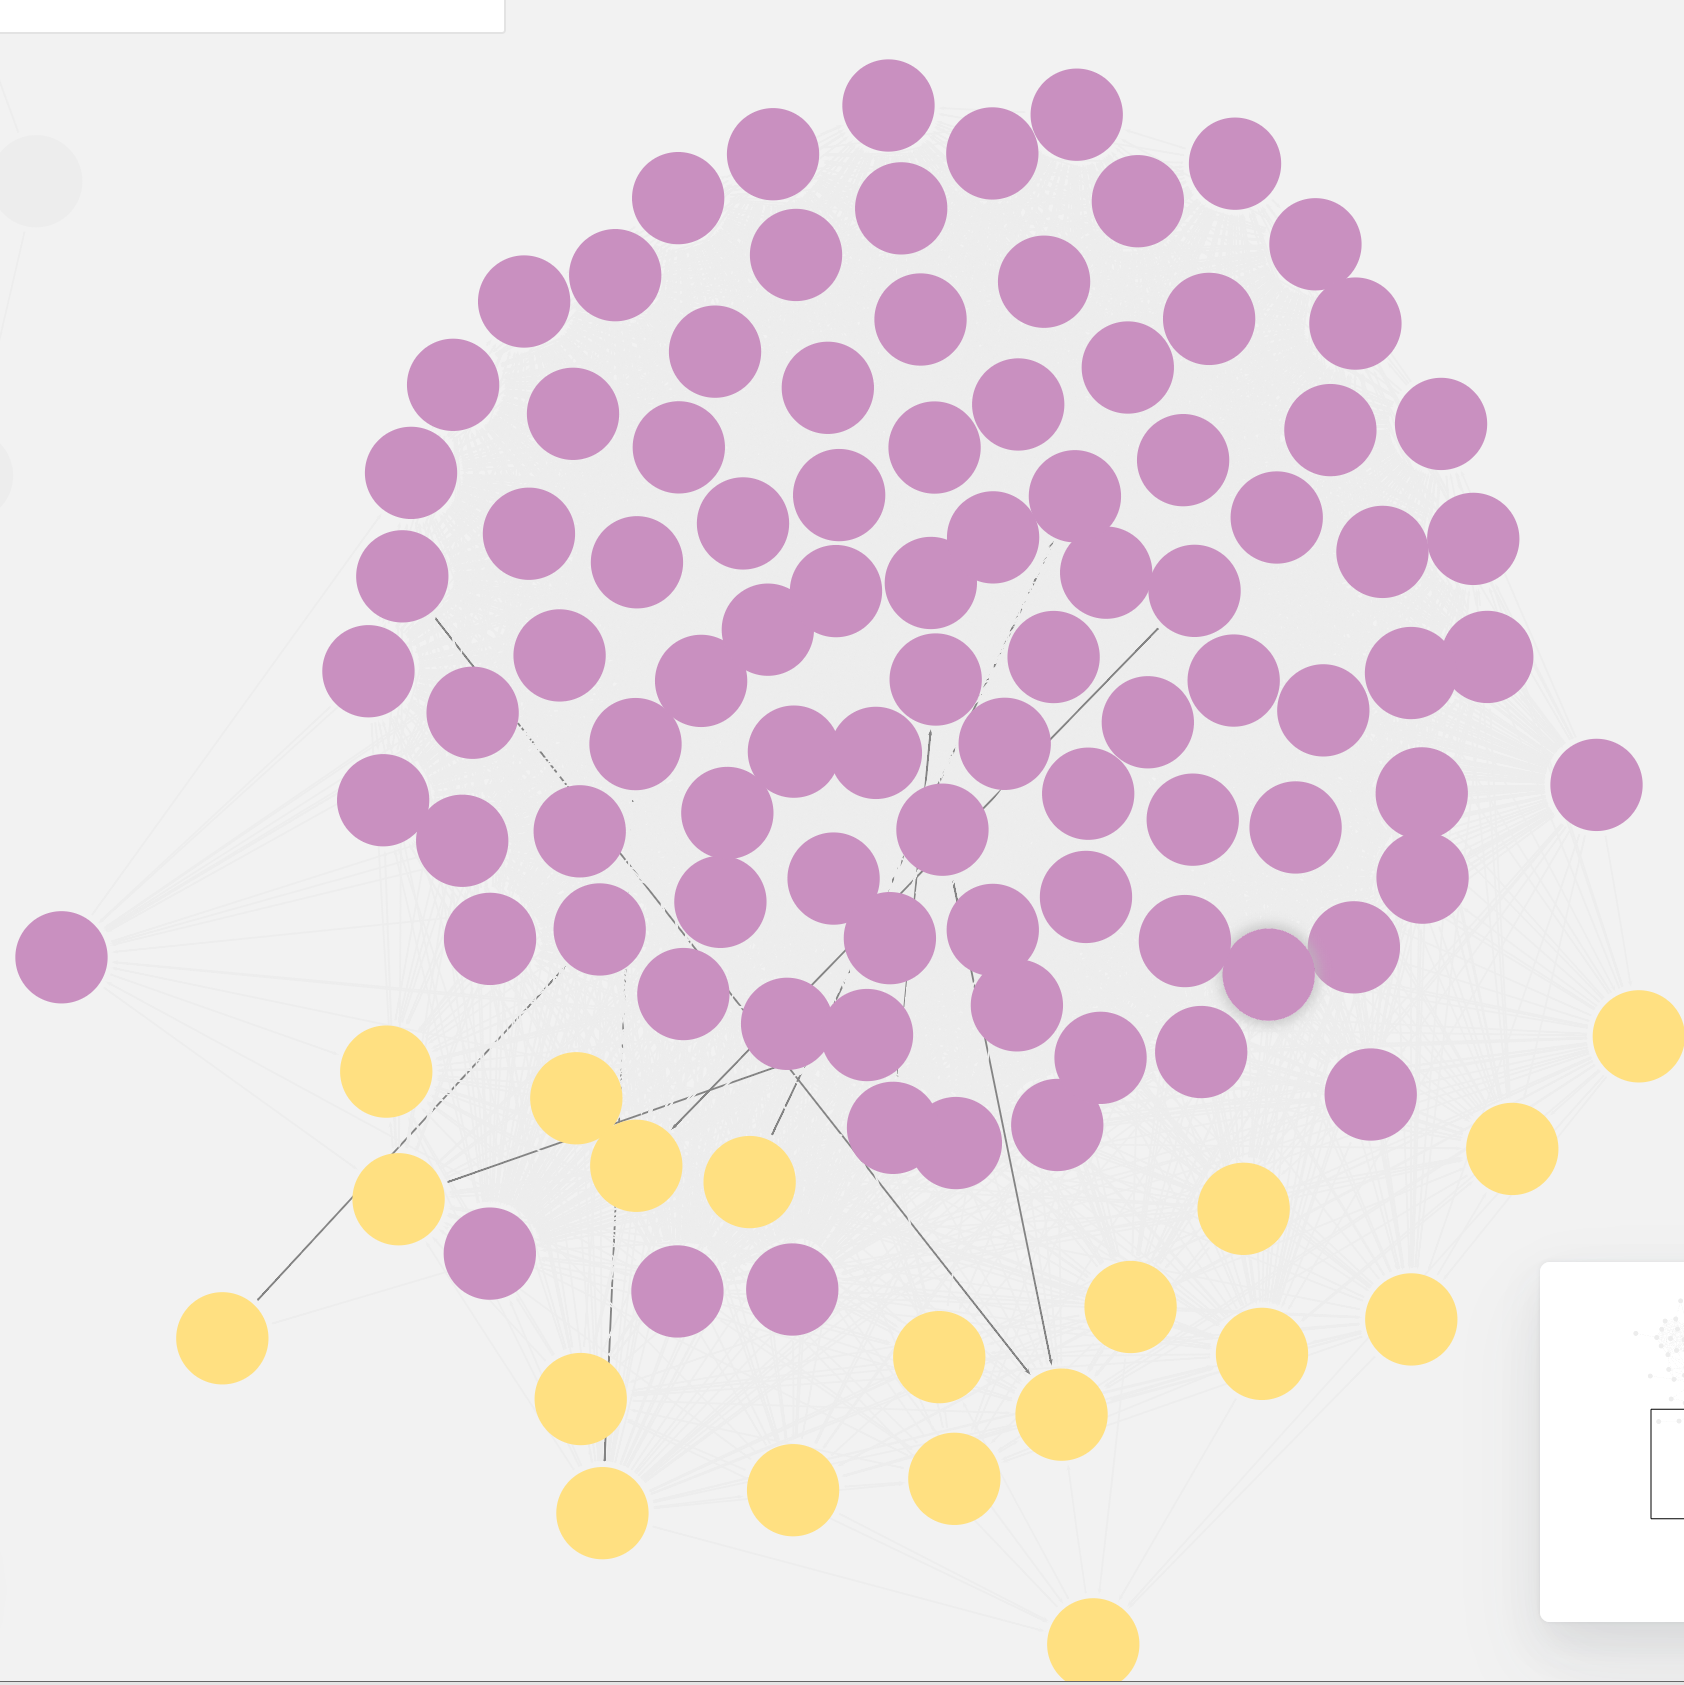
\includegraphics[]{img/only12.png}}
    \caption{\scriptsize Graph with edges of Type 1,2}
    \label{subfig:ab12}
  \end{subfigure}
  \begin{subfigure}[t]{.15\linewidth}
    \resizebox{\linewidth}{!}{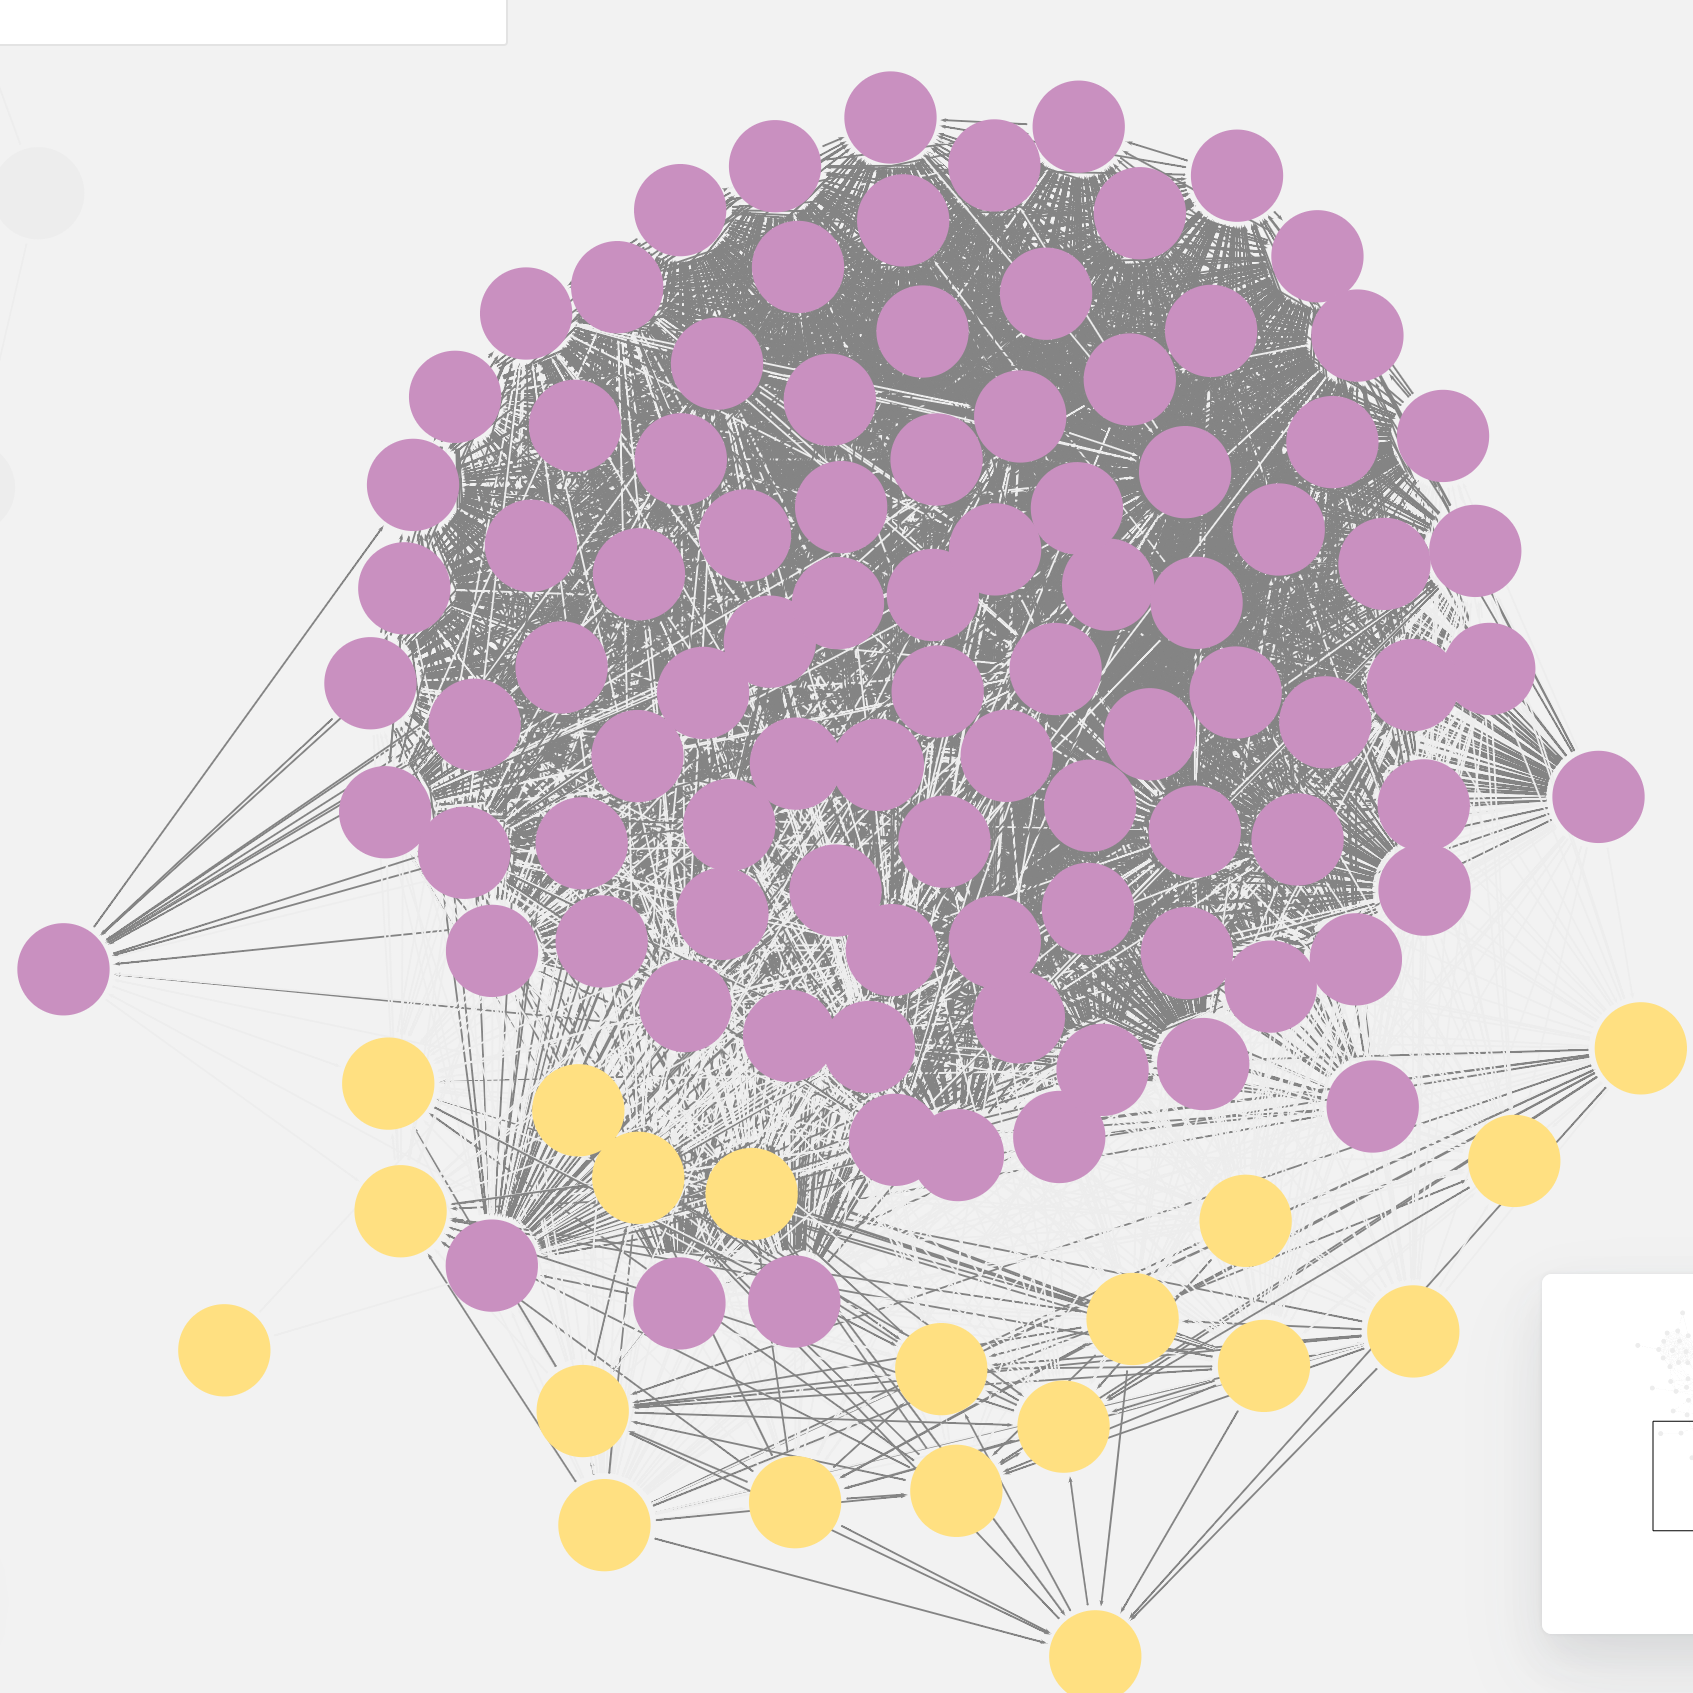
\includegraphics[]{img/only124.png}}
    \caption{\scriptsize Graph with edges of Type 1,2,4}
    \label{subfig:ab124}
  \end{subfigure}
  \begin{subfigure}[t]{.15\linewidth}
    \resizebox{\linewidth}{!}{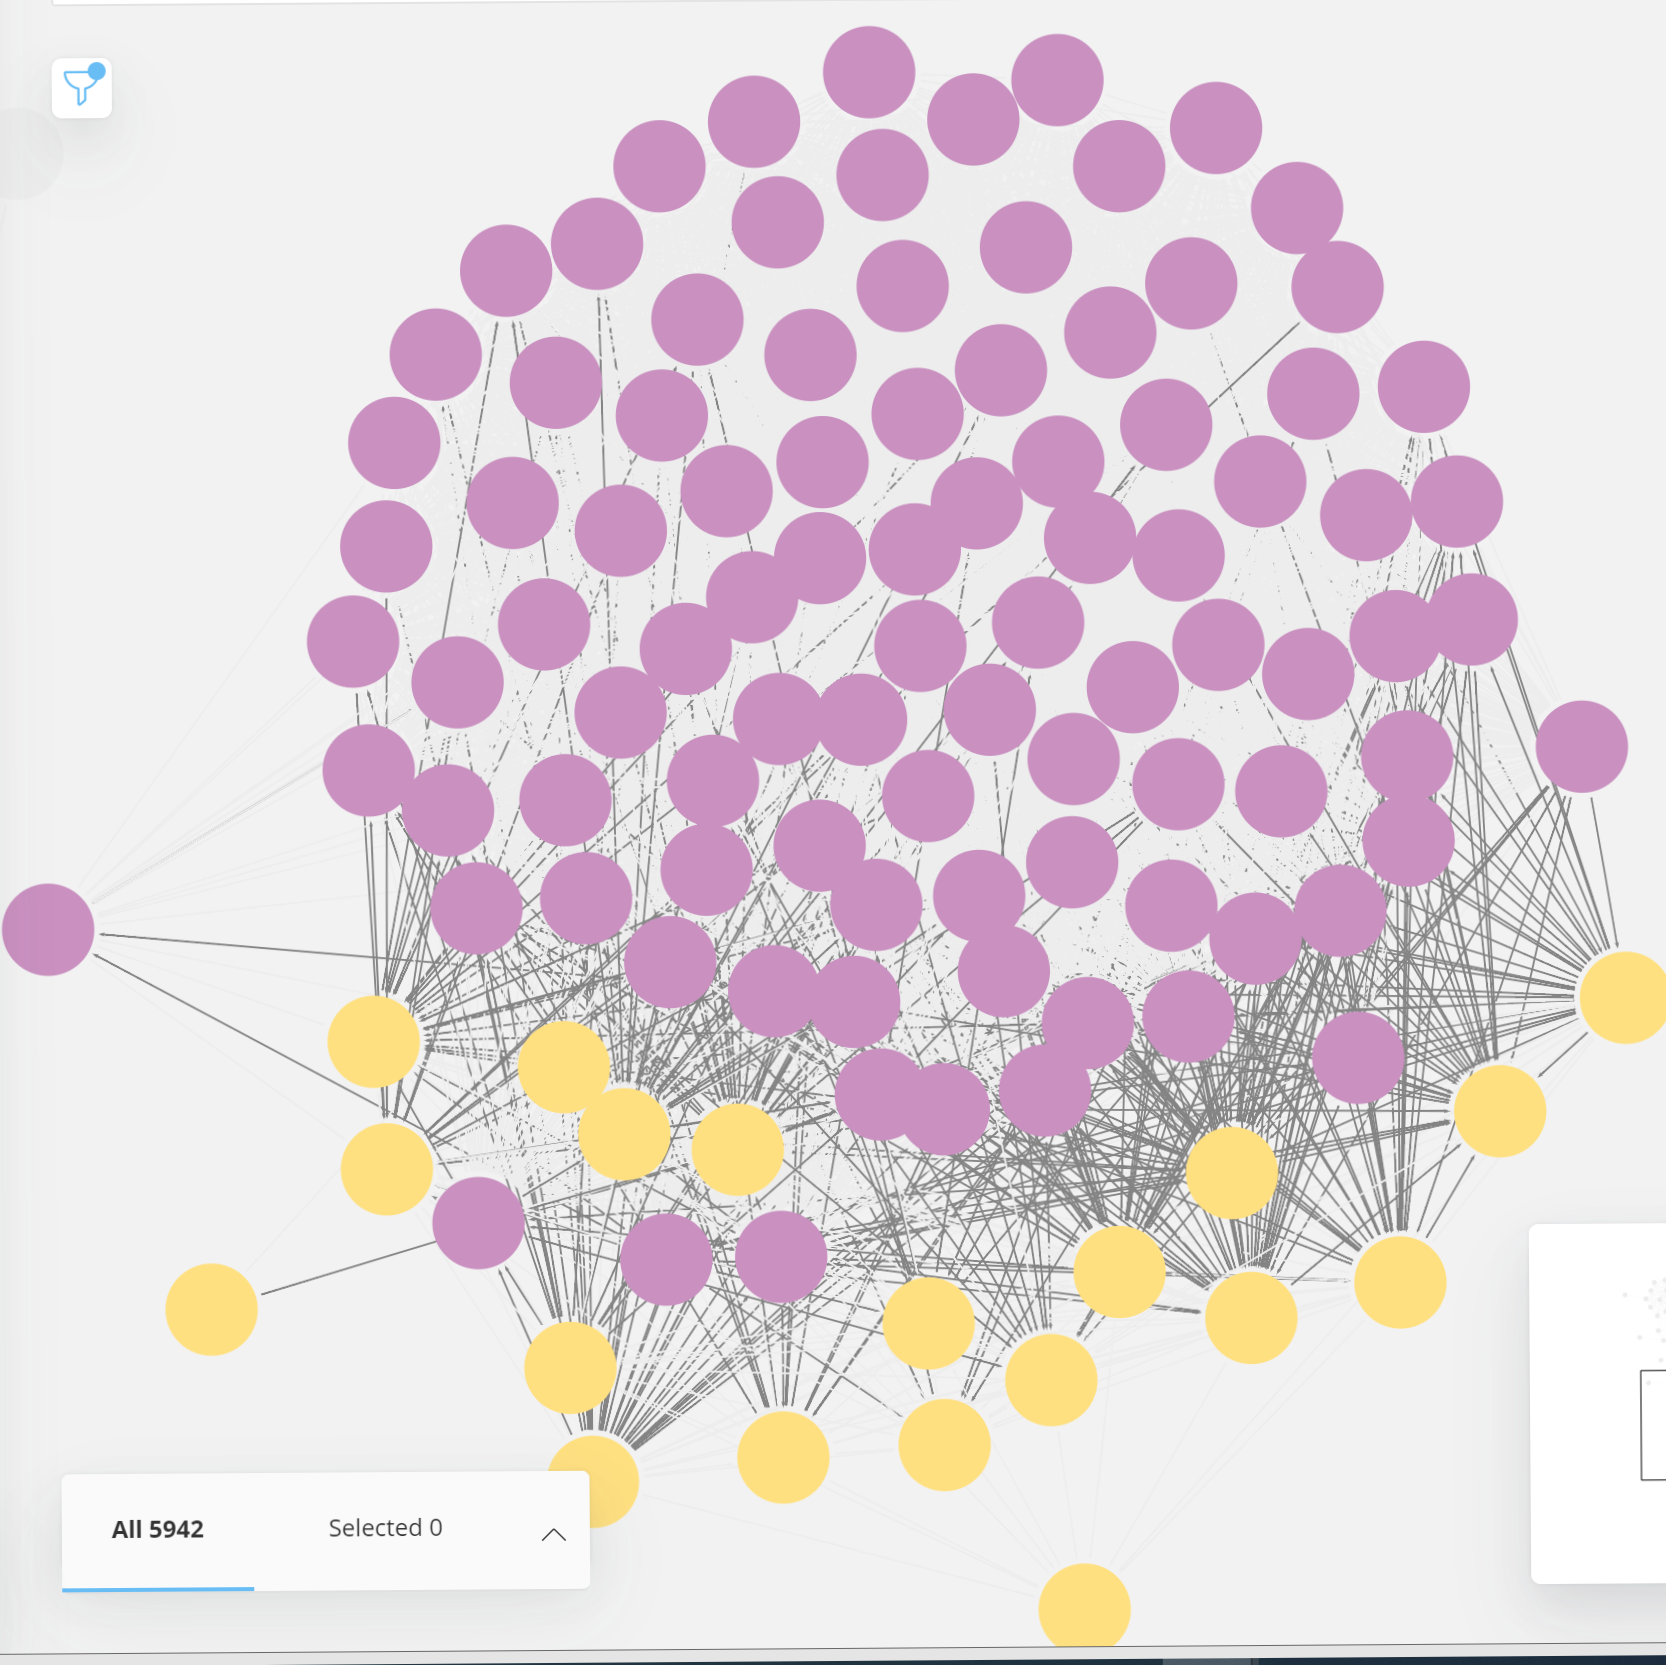
\includegraphics[]{img/only3.png}}
    \caption{\scriptsize Graph with edges of Type 3}
    \label{subfig:ab3}
  \end{subfigure}
    \caption{Ablation study on Relational sentence graph. {Violet nodes} are non-biased, {Yellow nodes} are biased.}
    \label{fig:ablation}
  \end{figure*}
  

\begin{table*}[th]
  \centering \scriptsize
    \begin{tabular}{p{4em}p{5em}p{5em}p{5em}p{5em}p{5em}p{6em}p{5em}}
    \toprule[2pt]
         \textbf{Variant} & \textbf{MultiCTX} & \textbf{CSE + BiLSTM} & \textbf{Discourse relationship } & \textbf{Semantic similarity} & \textbf{Event-context} & \textbf{Neighborhood-context}  &  \textbf{w/o Entity continuation} \\\midrule[1pt]
        %  w/ or w/o &  &  &  only  & only   & w/o  & only &  w/o \\ \midrule
        %  \multicolumn{5}{l}{$^${*} All results are implemented or reproduced by ourselves except for the second EvCIM record}
        %  without &  &  & Semantic similarity &  & Adjacent sentences &  &  Entity continuation  \\ \hline
       Edge types &  1,2,3,4  & No graph & 1,2,3 & 4  & 3,4 &  1,2 & 1,2,4\\\hline
      %  Context level &  Neighborhood + Event &  & Neighborhood + Event & Event  & Event &  Neighborhood & Neighborhood + Event \\\hline
    Precision &    $47.78 \pm 0.94$   &  $48.53 \pm 0.73$ &  $47.43 \pm 0.96$ &    $47.16 \pm 0.27$   &  $47.07\pm 0.99$ &  $47.18 \pm 1.08$     &  $47.56 \pm 0.62$       \\
    \hline
    Recall &   $44.50 \pm 0.65$    &   $41.98\pm 0.36$  & $44.39\pm 0.84$  &    $43.47\pm 0.38$ & $44.64\pm 0.37$  & $44.01\pm 0.91$  &      $43.72\pm 0.76$   \\
    \hline
    F1    &  $46.08\pm0.21$  & $45.01 \pm 0.26 $  &   $45.85\pm0.35$    &  $45.24\pm0.18$        & $45.81\pm0.42 $     & $45.53\pm0.29$   &  $45.55\pm0.34$\\
    \bottomrule[2pt]
    \end{tabular}%
      \caption{Ablation study on different types of edges in SSGAT. Mean and standard deviation across 5 seeds are reported. \KZ{Why don't you show
all types, all - 1, all -2, all -3, etc? The combination you provided here
look a bit arbitrary and could be objected to by people.}}
  \label{tab:ablation}%
\end{table*}%


  
Table \ref{tab:ablation} shows the ablation results. We can conclude that, 

\begin{itemize}
    \item \textbf{Context information transfers via edges in graph is better than via cells in BiLSTM. }
    
    All variants with graphs have better F1 score than the model without graph (CSE+BiLSTM, F1=45.01). 
    
    Figure \ref{fig:ablation} shows graphs with different edges in our ablation study using a subgraph of one event. {Violet nodes} are non-biased sentences, {Yellow nodes} are biased sentences.
    
    \item \textbf{Discourse relationship contributes more than semantic similarity to SSGAT.} SSGAT with only discourse relationships (F1=45.85) still has close performance to the full MultiCTX, while SSGAT with only semantic similarity edges (F1=45.25) suffers a considerable decrease in its performance. Note that the semantic similarity is calculated based on CSEs, so SSGAT with only such edges didn't add much extra information but may introduce duplication. It can be explained by Figure \ref{subfig:ab4}: connections are mostly within non-based words while inter-communication between biased/non biased nodes are more frequent in Figure \ref{subfig:ab123}.
    
    % edges of Therefore, edges connected by semantic similarity and by discourse relationships may overlap partially.
    
    % Note that the semantic similarity is calculated based on CSEs, and CSEs are learnt from article and event contexts encoded by triplets. Therefore, edges connected by semantic similarity and by discourse relationships may overlap partially.

    \item \textbf{Event-level context is more important than neighborhood-level context.} While they are both important according to our results, global event-level context contributes more than local neighborhood-level context. SSGAT with only adjacent sentences (Type 1,2) obtains F1=45.53 and with only Type 3,4 gets F1=45.81. The result is intuitive because edges of type 3,4 not only include adjacent sentences within article, but also extend to the whole event. We can also see the rare presence of edges of Type 1,2 in Figure \ref{subfig:ab12} compared with the closely linked graph in Figure  \ref{subfig:ab34}.

    \item \textbf{Adjacent sentences encoded by graph better interprets context information than brute-force PLMs.} In terms of neighborhood-level context, our SSGAT beats WinSSC by increasing massively the F1 score from F1=37.58 (Table \ref{tab:res}) to F1=45.53. 
    
    
    \item \textbf{Entity continuation is the most important edge type.} Among three ablation experiments removing respectively edges of Type 4 (F1=45.85), Type 1,2 (F1=45.81) and Type 3 (F1=45.55), the last one without Type 3 (entity continuation) suffers the largest performance drop. It suggests that entity continuation, or, coreference is the most important relation in our setting.
    We can clearly see that Type 3 edges are the main reason for inter-class communication from Figure \ref{subfig:ab3}.

\end{itemize}



\section{Related Work}

\paragraph{Media bias Detection.} 
% Datasets for media bias detection are limited and not standardized since it requires heavy workloads for humans to annotate manually the subtle bias with certain level of expertise. Besides, human annotators can suffer from implicit media bias and their judgments are subjective as well. However, there are still some sentence-level media bias datasets. \citet{wei2020newb} proposed a large sentence-level corpus for political bias detection, \citet{lim-etal-2020-annotating} proposed a sentence-level media bias dataset of 996 sentences from 46 news articles covering 4 topics, \citet{10.1145/3366423.3380158} further built a dataset consisting of more than 2000 sentences annoted with 43000 bias including subjectivity, hidden assumptions and representation tenddencies, \citet{spinde2021mbic} also created a sentence-level media bias dataset with the emphasis on annotators' backgrounds, \citet{fan-etal-2019-plain} presented the BASIL dataset used in our study.

% Linguistic features-based techniques are initially utilized in media bias detection and they are still widely applied till today because they provide a strong descriptive and explanatory power. These techniques are systematically formulated in \citep{recasens-etal-2013-linguistic}. \citep{chen-etal-2020-analyzing} explored linguistic patterns at word-level and article-level to analyze political bias in news articles; \citet{SPINDE2021102505} engineered various linguistic, lexical and syntactic features to detect media bias; \citet{10.1145/3366423.3380158} made used of syntactic structure to obtain generalized text embedding for news credibility check; and \citet{baly-etal-2019-multi} used a multi-task ordinal regression framework.

With the rise of deep learning, neural-based aproaches are broadly used in media bias detection. \citet{iyyer-etal-2014-political} used RNNs to aggregate
the polarity of each word to predict political ideology on sentence-level. \citet{gangula-etal-2019-detecting}
made use of headline attention to classify article
bias. \citet{li-goldwasser-2019-encoding} captured social information by Graph Convolutional Network to identify political bias in news articles. \citet{fan-etal-2019-plain} used BERT and RoBERTa and \citet{van-den-berg-markert-2020-context} used BiLSTMs as well as BERT-based models to detect sentence-level informational bias.
\paragraph{Contextual information in media bias detection.} 
Contextual information is explored, though primarily, in media bias detection. \citet{baly2020detect} employed an adversarial news media adaptation using triplet loss; \citet{kulkarni-etal-2018-multi} proposed an attention based model to capture views from news articles' title, content and link structure; \citet{chen-etal-2020-detecting} explored the impact of sentence-level bias to article-level bias; \citet{li-goldwasser-2019-encoding} encoded social information using GCN; \citet{baly-etal-2018-predicting} made use of news media's cyber-features in news factuality prediction; \citet{10.1145/3366423.3380158} explored cross-media context by a news article graph.

Sentence-level informational bias is under-studied by only a few research and the methods described above are not applicable on this task. In order to infuse contextual information, we refer to extractive summarization \citet{10.1145/3397271.3401327} and \citet{christensen-etal-2013-towards} which used sentence graph to encode context.

% extractive summarization
% \paragraph{Contrastive learning}
% \paragraph{Graph Attention Network}
\section{Conclusion}

We proposed MultiCTX, a model composed of contrastive learning 
and relational sentence graph attention network to encode such multi-level context at different stages.
Our model not only significantly outperforms the current 
state-of-the-art model. Therefore, we conclude that our model 
successfully learns from contextual information and 
that multi-level contextual information can effectively improves 
the identification of sentence-level informational bias. 

% 成功encode了context

    % Due to unavoidable non-deterministic atomic operations in implementation, the result here may cannot be reproduced exactly, but we took an average on our experiments to reflect its range. Also 
\bibliography{aaai22.bib}

\end{document}





